\exercisesection{5}

\begin{enumerate}
\def\labelenumi{\arabic{enumi}.}
\tightlist
\item
令 A 为交换环，\(\mathfrak{I}\) 为 A 的一个理想。称 A-模 M 关于 \(\mathfrak{I}\) 是绝对 Hausdorff 的，是指对于每个有限生成的 A-模 N，A-模 N \(\otimes_{\mathrm{A}}\) M 关于 \(\mathfrak{I}\) -进拓扑都是 Hausdorff 的；绝对 Hausdorff 的 A-模称为理想 Hausdorff 模。
\end{enumerate}

\begin{enumerate}
\def\labelenumi{(\alph{enumi})}
\item
M 关于 \(\mathfrak{I}\) 是绝对 Hausdorff 的充要条件是：对于每个有限生成的 A-模 N 及 N 的每个子模 \(\mathbf{N}'\)，\(\operatorname{Im}(\mathbf{N}' \otimes_{\mathbf{A}} \mathbf{M})\) 在 \(\mathbf{N} \otimes_{\mathbf{A}} \mathbf{M}\) 的 \(\mathfrak{I}\) -进拓扑下是闭的。
\item
  设 B 是交换的 A-代数，\(\mathfrak{L}\) 是 B 的一个包含 \(\mathfrak{I}B\) 的理想。如果 M 是关于 \(\mathfrak{L}\) 绝对 Hausdorff 的 B-模，则 M 是关于 \(\mathfrak{I}\) 绝对 Hausdorff 的 A-模。
\end{enumerate}

\begin{enumerate}
\def\labelenumi{\arabic{enumi}.}
\setcounter{enumi}{1}
\item
  证明每个关于 p-进拓扑为 Hausdorff 的 Z-模（p 为素数）都是理想 Hausdorff 模；但给出一个关于 p 为 Hausdorff 而非绝对 Hausdorff 的有限生成 Z-模的例子（使用习题 1 (a)）。
\item
用第 3 节习题 11 的记号。设 N 是 \(\hat{\mathbf{E}}\) 的子模，它是 \(\hat{\mathbf{E}}\) 中由 \(\hat{\mathbf{E}}\) 的子模所生成的向量 \(pe_{2n-1} - p^n e_{2n} (n \geqslant 1)\) 的闭包；令 M = \(\hat{\mathbf{E}}/\mathbf{N}\)。证明在 \(p\) -进拓扑下，M 的子模 \(p\mathbf{M}\) 在 M 中不是闭的，并由此推出 M 是理想 Hausdorff 的 \(\mathbf{Z}_p\)-模，但关于 \(p\) 不是绝对 Hausdorff 的。
\end{enumerate}

¶ 4. 设 A 为交换环，\(\mathfrak{I}\) 为 A 的一个理想，且 S = 1 + \(\mathfrak{I}\)。证明，如果 A-模 M 关于 \(\mathfrak{I}\) 是绝对 Hausdorff 的，则 S \(^{-1}\) M = M，换言之，对于所有 \(a \in\) S，\(x \mapsto ax\) 是 M 到自身的双射。（先证明 M 关于 \(\mathfrak{I}\)-进拓扑为 Hausdorff 的假设蕴含 \(x \mapsto ax\) 是单射；然后证明 M 的子模 aM 关于 \(\mathfrak{I}\)-进拓扑在 M 中稠密，并使用习题 1 (a)。）

\begin{enumerate}
\def\labelenumi{\arabic{enumi}.}
\setcounter{enumi}{4}
\tightlist
\item
  取 \(\mathbf{A} = \mathbf{Z}\) 及 \(\mathfrak{I} = p\mathbf{Z}\)，其中 \(p\) 为素数。
\end{enumerate}

\begin{enumerate}
\def\labelenumi{(\alph{enumi})}
\item
  证明，如果 \(q\) 是不同于 \(p\) 的素数，则 \(\mathbf{Z}\)-模 \(\mathbf{Z} / q\mathbf{Z}\) 满足定理 1 的性质 (ii)，但不满足性质 (i)。
\item
  证明 \(\mathbf{Z}\)-模 \(\mathbf{Q} / \mathbf{Z}\) 满足定理 1 的性质 (iv)，但不满足性质 (ii)。
\end{enumerate}

\begin{enumerate}
\def\labelenumi{\arabic{enumi}.}
\setcounter{enumi}{5}
\tightlist
\item
  设 A 是交换诺特环，\(\mathfrak{I}\) 是 A 的一个理想，M 是一个 A-模。证明定理 1 的条件 (v) 等价于下述条件：
\end{enumerate}

(v') 对于每个有限生成的 A-模 N 及 N 的每个子模 N'，典范映射 \((\mathbf{M} \otimes_{\mathbf{A}} \mathbf{N}')^{\wedge} \to (\mathbf{M} \otimes_{\mathbf{A}} \mathbf{N})^{\wedge}\) 是单射（其中两边分别是 M \(\mathfrak{I}\) 和 M \(\otimes_{A} N'\) 上的 \(\otimes_{A} N\) -进拓扑所对应的 Hausdorff 完备化）。（证明 (v) 蕴含 (v') 时，仿照定理 1 的证明中部分 (E) 的论证。为看出 (v') 蕴含 (v)，考虑被 \(\mathfrak{I}\) 的某个幂湮灭的 A-模 N。）

¶ 7. 设\((A_{\lambda}, f_{\mu\lambda})\)是诺特局部环的有向直接系统；若\(m_{\lambda}\)是\(A_{\lambda}\)的极大理想，假设对于\(\lambda \leqslant \mu\)，有\(m_{\mu} = m_{\lambda}A_{\mu}\)且\(A_{\mu}\)是平坦的\(A_{\lambda}\)。证明\(A = \lim A_{\lambda}\)是诺特环，并且对于所有\(A_{\lambda}\)都是平坦的\(\lambda\)。（若\(m = m_{\lambda}A\)是\(A\)的极大理想（第二章，第 3 节，习题 16），证明在\(A\)上 m-进拓扑是 Hausdorff 的，注意到\(A\)是忠实平坦的\(A_{\lambda}\)对于所有\(\lambda\)。（然后证明，若\(\hat{A}\)是\(A\)关于 m-进拓扑的完备化，则\(\hat{A}\)是诺特环；利用 § 2，第 10 节定理 2 的推论 5；最后证明，对于所有\(\lambda\)，\(\hat{A}\)都是平坦的\(A_{\lambda}\)-模，利用第 2 节定理 1 和第 3 节命题 2。）

¶ 8. 设 A 是诺特局部环，m 是其极大理想，k = A/m 是其剩余域。设 K 是 k 的一个扩域；证明存在从 A 到某个诺特局部环 B 的局部同态，使得 B/mB 同构于 K，且 B 是平坦的 A-模。（先考虑 \(\mathbf{K} = k(t)\) 的情形，根据 t 在 k 上是代数的还是超越的分两种情况；再考虑 K 的包含 k 的子域族 \((\mathrm{K}_{\lambda})\)，该族按包含关系良序，且若 \(K_{\lambda}\) 有前驱 \(\mathrm{K}_{\mu}, \mathrm{K}_{\lambda} = \mathrm{K}_{\mu}(t_{\mu})\)，其中 \(t_{\mu} \in K_{\mu}\)；最后应用习题 7。）

第 IV 章(*)

\chapter{伴随素理想与准素分解}

(*) 本章的结果只依赖于本书第一至第六卷以及第一至第三章，不包括第一章第 4 节和第三章第 5 节。

本章所考虑的所有环都假设为交换环并具有单位元；所有环同态都假设把单位元映到单位元。环 A 的子环是指包含 A 的单位元的子环。

回忆一下，对于每个 A-模 E 及所有 \(x \in E\)，\(\text{Ann}(x)\) 表示 x 的湮灭子，即满足 ax = 0 的 \(a \in A\) 所成的集合。

\section{与模相伴的素理想}

\subsection{伴随素理想的定义}

定义 1. 设 M 是环 A 上的模。如果存在 \(x \in M\)，使得 p 等于 x 的湮灭子，则称素理想 p 与 M 相伴。与 M 相伴的素理想所成的集合记为 \(\operatorname{Ass}_{\mathbf{A}}(\mathbf{M})\)，或简称为 \(\operatorname{Ass}(\mathbf{M})\)。

* 例。设 \(a\) 是多项式环 \(A = \mathbf{C}[X_1, \ldots, X_r]\) 中的一个理想，\(V\) 是相应的仿射代数簇，\(V_1, \ldots, V_p\) 是 \(V\) 的不可约分支。若取 \(M\) 为在 \(A/a\) 上正则的函数环 \(V\)，则与 \(M\) 相伴的素理想集合由 \(V_1, \ldots, V_p\) 的理想以及一般还包括其他素理想组成，后者中的每一个都包含某个 \(V_1\) 的理想。

由于 0 的湮灭子是 A，湮灭子为素理想的元素 \(x \in \mathbf{M}\) 必然满足 \(\neq 0\)。称素理想 \(p\) 与 M 相伴，等价于说 M 含有一个同构于 A/p 的子模（即对于湮灭子为 p 的所有 \(x \in M\)，子模 Ax）。

如果 A-模 M 是子模族 \((M_{t})_{t\in I}\) 的并，则显然

\[
\operatorname{Ass} (\mathbf {M}) = \bigcup_ {\iota \in I} \operatorname{Ass} \left(\mathbf {M} _ {\iota}\right).\tag{1}
\]

命题 1. 对于每个素理想 \(\mathfrak{p}\)（在环 \(\mathbf{A}\) 中）以及 \(\mathbf{M} \neq 0\) 的每个子模 \(\mathbf{A} / \mathfrak{p}\)，都有 \(\operatorname{Ass}(\mathbf{M}) = \{\mathfrak{p}\}\)。

由于环 A/p 是整环，A/p 中任一元素 \(\neq0\) 的湮灭子都是 p。

命题 2. 设 M 是环 A 上的模。由 M 中所有元素 \(\neq0\) 所对应的 A 的理想 Ann(x) 构成的集合的每个极大元都属于 Ass(M)。

令 \(\mathfrak{a} = \operatorname{Ann}(x)\) ( \(x \in \mathbf{M}, x \neq 0\) ) 为这样的极大元；只需证明 \(\mathfrak{a}\) 是素理想。由于 \(x \neq 0\)，\(\mathfrak{a} \neq \mathbf{A}\)。设 \(b, c\) 是 \(\mathbf{A}\) 中满足 \(bc \in \mathfrak{a}\) 且 \(c \notin \mathfrak{a}\) 的元素。则 \(cx \neq 0\)，\(b \in \operatorname{Ann}(cx)\) 且 \(\mathfrak{a} \subset \operatorname{Ann}(cx)\)。由于 \(\mathfrak{a}\) 是极大的，\(\operatorname{Ann}(cx) = \mathfrak{a}\)，从而 \(b \in \mathfrak{a}\)，故 \(\mathfrak{a}\) 是素理想。

推论 1. 设 M 是诺特环 A 上的模。则条件 \(M \neq \{0\}\) 等价于 \(\operatorname{Ass}(M) \neq \varnothing\)。

如果 \(M = \{0\}\)，显然 \(\text{Ass}(M)\) 为空（对 A 不需作任何假设）。如果 \(M \neq \{0\}\)，则形如 \(\text{Ann}(x)\)（其中 \(x \in M\) 且 \(x \neq 0\)）的理想所成的集合非空，且其中的理想都满足 \(\neq A\)；由于 A 是诺特环，该集合有极大元；于是只需应用命题 2。

推论 2. 设 A 是诺特环，M 是 A-模，a 是 A 的元素。M 上比为 a 的伸缩映射为单射的充要条件是：a 不属于任何与 M 相伴的素理想。

如果 \(a\) 属于素理想 \(\mathfrak{p} \in \operatorname{Ass}(\mathbf{M})\)，则 \(\mathfrak{p} = \operatorname{Ann}(x)\)，其中 \(x \in \mathbf{M}\)，\(x \neq 0\)；于是 \(ax = 0\)，乘为 \(a\) 的伸缩映射不是单射。反之，若 \(ax = 0\) 对某个 \(x \in \mathbf{M}\) 且 \(x \neq 0\) 成立，则 \(Ax \neq \{0\}\)，从而 \(\operatorname{Ass}(x) \neq \varnothing\)（推论 1）。令 \(\mathfrak{p} \in \operatorname{Ass}(\mathbf{A}x)\)；则显然 \(\mathfrak{p} \in \operatorname{Ass}(\mathbf{M})\)，且 \(\mathfrak{p} = \operatorname{Ann}(bx)\)，其中 \(b \in \mathbf{A}\)；故 \(a \in \mathfrak{p}\)，因为 \(abx = 0\)。

推论 3. 诺特环 A 中的零因子集合是理想 \(\mathfrak{p} \in \operatorname{Ass}(A)\) 的并。

命题 3. 设 A 是一个环，M 是一个 A-模，N 是 N 的子模。则

\[
\operatorname{Ass} (\mathbf {N}) \subset \operatorname{Ass} (\mathbf {M}) \subset \operatorname{Ass} (\mathbf {N}) \cup \operatorname{Ass} (\mathbf {M} / \mathbf {N}).\tag{2}
\]

包含关系 \(\operatorname{Ass}(\mathbf{N}) \subset \operatorname{Ass}(\mathbf{M})\) 显然。设 \(\mathfrak{p} \in \operatorname{Ass}(\mathbf{M})\)，\(\mathbf{E}\) 是 \(\mathbf{M}\) 中同构于 \(\mathbf{A} / \mathfrak{p}\) 的子模，且 \(\mathbf{F} = \mathbf{E} \cap \mathbf{N}\)。若 \(\mathbf{F} = \{0\}\)，则 \(\mathbf{E}\) 同构于 M/N 的一个子模，从而 \(\mathfrak{p} \in \operatorname{Ass}(M/N)\)。若 \(F \neq \{0\}\)，则 F 中每个元素 \(\neq 0\) 的湮灭子都是 p（命题 1），因而 \(\mathfrak{p} \in \operatorname{Ass}(F) \subset \operatorname{Ass}(N)\)。

推论 1. 如果 A-模 M 是子模族 \((\mathbf{M}_t)_{t \in I}\) 的直和，则 \(\operatorname{Ass}(\mathbf{M}) = \bigcup_{t \in I} \operatorname{Ass}(\mathbf{M}_t)\)。

由 (1) 可将其归结为 I 是有限集的情形，再通过对\(\operatorname{Card}(I) = 2\)归纳将其归结为\(\operatorname{Card}(I)\)的情形。令\(I = \{i, j\}\)，其中\(i \neq j\)；由于\(M/M_{i}\)同构于\(M_{j}\)，\(\operatorname{Ass}(M) \subset \operatorname{Ass}(M_{i}) \cup \operatorname{Ass}(M_{j})\)（命题 3）；此外，\(\operatorname{Ass}(M_{i})\)和\(\operatorname{Ass}(M_{j})\)都包含于\(\operatorname{Ass}(M)\)（命题 3），结论得证。

推论 2. 设 M 是 A-模，\((\mathbf{Q}_i)_{i\in I}\) 是 M 的有限个子模组成的族。若 \(\bigcap_{i\in I} \mathbf{Q}_i = \{0\}\)，则

\[
\operatorname{Ass} (\mathbf {M}) \subset \bigcup_ {i \in I} \operatorname{Ass} (\mathbf {M} / \mathbf {Q} _ {i}).
\]

典范映射 \(\mathbf{M} \to \bigoplus_{i \in I} (\mathbf{M} / \mathbf{Q}_i)\) 是单射；于是只需应用命题 3 及其推论 1。

命题 4. 设 M 是 A-模，\(\Phi\) 是 \(\operatorname{Ass}(\mathbf{M})\) 的子集。则存在 M 的一个子模 N，使得 \(\operatorname{Ass}(\mathbf{N}) = \operatorname{Ass}(\mathbf{M}) - \Phi\) 且 \(\operatorname{Ass}(\mathbf{M}/\mathbf{N}) = \Phi\)。

令\(\mathfrak{E}\)为 M 的子模\(P\)的集合，满足\(M\)。公式 (1) 表明，按包含关系排序的集合\(\operatorname{Ass}(P) \subset \operatorname{Ass}(M) - \Phi\)是归纳的；此外，\(\mathfrak{E}\)，因而\(\{0\} \in \mathfrak{E}\)。令\(\mathfrak{E} \neq \varnothing\)为\(N\)的极大元。则\(\mathfrak{E}\)。我们将看到\(\operatorname{Ass}(N) \subset \operatorname{Ass}(M) - \Phi\)，命题 3 将完成证明。设\(\operatorname{Ass}(M/N) \subset \Phi\)；则\(p \in \operatorname{Ass}(M/N)\)含有一个子模\(M/N\)同构于\(F/N\)。由命题 1 和命题 3，\(A/p\)。由于\(\operatorname{Ass}(F) \subset \operatorname{Ass}(N) \cup \{p\}\)是\(N\)中的极大元，\(\mathfrak{E}\)不属于\(F \notin \mathfrak{E}\)，从而\(p \in \Phi\)。

\subsection{伴随素理想的局部化}

命题 5. 设 A 是环，S 是 A 的乘性子集，\(\Phi\) 是 A 中不与 S 相交的素理想集合，M 是 A-模。则：

\begin{enumerate}
\def\labelenumi{(\roman{enumi})}
\item
  \(\mathfrak{p} \mapsto \mathrm{S}^{-1}\mathfrak{p}\) 是从 \(\operatorname{Ass}_{\mathbf{A}}(\mathbf{M}) \cap \Phi\) 到 \(\operatorname{Ass}_{\mathbf{S}^{-1}\mathbf{A}}(\mathbf{S}^{-1}\mathbf{M})\) 的某个子集的双射。
\item
  如果 \(\mathfrak{p} \in \Phi\) 是有限生成理想，且 \(S^{-1}\mathfrak{p} \in \operatorname{Ass}_{\mathbf{S}^{-1}\mathbf{A}}(\mathbf{S}^{-1}\mathbf{M})\)，则 \(\mathfrak{p} \in \operatorname{Ass}_A(M)\)。
\end{enumerate}

回忆（第二章，第 2 节，第 5 节，命题 11），映射\(\mathfrak{p} \mapsto \mathrm{S}^{-1}\mathfrak{p}\)是从\(\Phi\)到\(\mathrm{S}^{-1}\mathrm{A}\)的素理想集合的双射。如果\(\mathfrak{p} \in \operatorname{Ass}_{\mathbf{A}}(\mathbf{M}) \cap \Phi\)，则\(\mathfrak{p}\)是\(\mathbf{N}\)的一个单生成子模\(\mathbf{M}\)的湮灭子；于是\(\mathrm{S}^{-1}\mathfrak{p}\)是\(\mathrm{S}^{-1}\mathrm{N}\)的单生成子模\(\mathrm{S}^{-1}\mathrm{M}\)的湮灭子（第二章，第 2 节，第 4 节，公式 (9)），从而\(\mathbf{S}^{-1}\mathfrak{p}\in\mathrm{Ass}_{\mathbf{S}^{-1}\mathbf{A}}(\mathbf{S}^{-1}\mathbf{M})\)。反之，设\(\mathfrak{p}\in\Phi\)是有限生成的，且\(\mathbf{S}^{-1}\mathfrak{p}\)与\(\mathbf{S}^{-1}\mathbf{M}\)相伴；则存在\(x\in\mathbf{M}\)和\(t\in\mathbf{S}\)，使得\(\mathbf{S}^{-1}\mathfrak{p}\)是\(x/t\)的湮灭子。设\((a_{i})_{1\leqslant i\leqslant n}\)是\(\mathfrak{p}\)的一组生成元；则\((a_{i}/1)(x/t)=0\)，从而存在\(s_{i}\in\mathbf{S}\)，使得\(s_{i}a_{i}x=0\)（\(1\leqslant i\leqslant n\)）。记\(s=s_{1}s_{2}\ldots s_{n}\)；对于所有\(a\in\mathfrak{p}\)，有\(sax=0\)，从而\(\mathfrak{p}\subset\mathrm{Ann}(sx)\)；另一方面，若\(b\in\mathbf{A}\)满足\(bsx=0\)，则按定义\(b/1\in\mathbf{S}^{-1}\mathfrak{p}\)，从而\(b\in\mathfrak{p}\)。于是\(\mathfrak{p}=\mathrm{Ann}(sx)\)，且\(\mathfrak{p}\in\mathrm{Ass}_{\mathbf{A}}(\mathbf{M})\)。

推论。若环 A 是诺特环，则映射 \(\mathfrak{p} \mapsto \mathrm{S}^{-1}\mathfrak{p}\) 是从 \(\operatorname{Ass}_{\mathbf{A}}(\mathbf{M}) \cap \Phi\) 到 \(\operatorname{Ass}_{\mathbf{S}^{-1}\mathbf{A}}(\mathbf{S}^{-1}\mathbf{M})\) 的双射。

若 A 不是诺特环，则从 \(p \mapsto S^{-1}p\) 的 \(\operatorname{Ass}_{\mathbf{A}}(\mathbf{M}) \cap \Phi\) 到 \(\operatorname{Ass}_{\mathbf{S}^{-1}\mathbf{A}}(\mathbf{S}^{-1}\mathbf{M})\) 的映射不一定是满射（习题 1）。

命题 6. 设 A 是诺特环，M 是 A-模，S 是 A 的乘性子集，\(\Psi\) 是 \(\operatorname{Ass}_{\mathbf{A}}(\mathbf{M})\) 中不与 S 相交的元素所成的集合。则典范映射 \(M \to S^{-1}M\) 的核 N 是 M 的唯一子模，满足下列关系

\[
\operatorname{Ass} (N) = \operatorname{Ass} (M) - \Psi , \quad \operatorname{Ass} (M / N) = \Psi .\tag{3}
\]

根据第 1 节命题 4，存在\(\mathbf{N}'\)是\(\mathbf{M}\)的子模，满足关系\(\operatorname{Ass}(\mathbf{N}') = \operatorname{Ass}(\mathbf{M}) - \Psi'\)以及\(\operatorname{Ass}(\mathbf{M}/\mathbf{N}') = \Psi'\)。我们需要证明\(\mathbf{N}' = \mathbf{N}\)。考虑交换图

\[
\begin{array}{c} \mathrm{M} \xrightarrow {p} \mathrm{M} / \mathrm{N} ^ {\prime} \\ u \Biggl \downarrow \\ \mathrm{S} ^ {- 1} \mathrm{M} \xrightarrow [ \mathrm{S} ^ {- 1 p} ]{} \mathrm{S} ^ {- 1} (\mathrm{M} / \mathrm{N} ^ {\prime}) \end{array}
\]

其中 \(p, u, v\) 是典范同态。我们将证明 \(S^{-1}p\) 和 \(v\) 是单射；这将证明 \(u\) 和 \(p\) 具有相同的核，从而 \(N' = N\)。

由于\(\operatorname{Ass}(\mathbf{N}') \cap \Psi' = \varnothing\)，\(\operatorname{Ass}(\mathbf{N}')\)的每个元素都与 S 相交。于是\(\operatorname{Ass}_{\mathbf{S}^{-1}\mathbf{A}}(\mathbf{S}^{-1}\mathbf{N}') = \varnothing\)（命题 5 的推论），从而\(\mathbf{S}^{-1}\mathbf{N}' = \{0\}\)（第 1 节命题 2 的推论 1），这说明\(\mathbf{S}^{-1}\mathfrak{p}\)是单射（第二章，第 2 节，第 4 节，定理 1）。另一方面，若\(x\)属于核 K 的\(v\)，则\(\operatorname{Ann}(x) \cap \mathbf{S} \neq \varnothing\)（第二章，第 2 节，第 2 节，命题 4）；于是\(\operatorname{Ass}(\mathbf{K}) = \varnothing\)，因为\(\operatorname{Ass}(\mathbf{K}) \subset \operatorname{Ass}(\mathbf{M}/\mathbf{N}') = \Psi'\)；我们推出\(\mathbf{K} = \{0\}\)（第 1 节命题 2 的推论 1），且\(v\)是单射。

\subsection{与支撑集的关系}

设 M 是环 A 上的模。回忆，A 的满足 \(M_{p} \neq 0\) 的素理想 p 所成的集合称为 M 的支撑集，记为 Supp(M)（第二章，第 4 节，第 4 节，定义 5）。

命题 7. 设 A 是环，M 是 A-模。

\begin{enumerate}
\def\labelenumi{(\roman{enumi})}
\item
A 的每个素理想 \(\mathfrak{p}\)，若包含 \(\operatorname{Ass}(\mathbf{M})\) 中的一个元素，则属于 \(\operatorname{Supp}(\mathbf{M})\)。
\item
反之，若 A 是诺特环，则每个理想 \(\mathfrak{p} \in \operatorname{Supp}(\mathbf{M})\) 都包含 \(\operatorname{Ass}(\mathbf{M})\) 中的一个元素。
\end{enumerate}

如果 \(\mathfrak{p}\) 包含 \(\mathfrak{q}\) 中的一个元素 \(\operatorname{Ass}(\mathbf{M})\)，则 \(\mathfrak{q} \cap (\mathbf{A} - \mathfrak{p}) = \varnothing\)，因此若记 \(\mathbf{S} = \mathbf{A} - \mathfrak{p}\)，则 \(\mathbf{S}^{-1}\mathfrak{p}\) 是与 \(\mathbf{S}^{-1}\mathbf{M} = \mathbf{M}_{\mathfrak{p}}\) 相伴的素理想（第 2 节，命题 5），特别地 \(\mathbf{M}_{\mathfrak{p}} \neq 0\)，从而 \(\mathfrak{p} \in \operatorname{Supp}(\mathbf{M})\)。反之，若 \(\mathbf{A}\) 是诺特环，则 \(\mathbf{A}_{\mathfrak{p}}\) 也是诺特环（第二章，第 2 节，第 4 节，命题 10 的推论 2）。若 \(\mathbf{M}_{\mathfrak{p}} \neq 0\)，则 \(\operatorname{Ass}_{\mathbf{A}_{\mathfrak{p}}}(\mathbf{M}_{\mathfrak{p}}) \neq 0\)（第 1 节，命题 2 的推论 1），所以存在 \(\mathfrak{q} \in \operatorname{Ass}_{\mathbf{A}}(\mathbf{M})\)，使得 \(\mathfrak{q} \cap (\mathbf{A} - \mathfrak{p}) = \varnothing\)（第 2 节，命题 5 的推论）。

推论 1. 如果 M 是诺特环上的模，则 \(\operatorname{Ass}(\mathbf{M}) \subset \operatorname{Supp}(\mathbf{M})\)，且这两个集合具有相同的极小元。

推论 2. 诺特环 A 的幂零根是理想 \(\mathfrak{p} \in \operatorname{Ass}(\mathbf{A})\) 的交。

我们知道，A 的幂零根是 \(\operatorname{Spec}(A) = \operatorname{Supp}(A)\) 的极小元的交（第二章，第 2 节，第 6 节，命题 13）。

\subsection{诺特环上的有限生成模情形}

定理 1. 设 A 是诺特环，M 是有限生成的 A-模。存在 M 的一个合成列 \((\mathbf{M}_i)_{0\leqslant i\leqslant n}\)，使得对于 \(0\leqslant i\leqslant n - 1\)，\(\mathbf{M}_i / \mathbf{M}_{i + 1}\) 同构于 \(\mathbf{A} / \mathfrak{p}_i\)，其中 \(\mathfrak{p}_i\) 是 A 的素理想。

令 \(\mathfrak{E}\) 为 M 的子模所成的集合，这些子模具有满足陈述的合成列。由于 \(\mathfrak{E}\) 非空（因为 \{0\} 属于 \(\mathfrak{E}\)），且 M 是诺特模，\(\mathfrak{E}\) 有极大元 N。若 M ≠ N，则 M/N ≠ 0，从而 \(\operatorname{Ass}(M/N) \neq \varnothing\)（第 1 节，命题 2 的推论 1）；因此 M/N 含有一个子模 N'/N，同构于形如 A/p 的 A-模，其中 p 是素理想；于是按定义 N' \(\mathfrak{E}\)，这与 N 的极大性矛盾。因此必有 N = M。

定理 2. 设 M 是诺特环 A 上的有限生成模，\((\mathbf{M}_{i})_{0\leqslant i\leqslant n}\) 是 M 的一个合成列，使得对于 \(0\leqslant i\leqslant n-1\)，\(M_{i}/M_{i+1}\) 同构于 \(A/p_{i}\)，其中 \(p_{i}\) 是 A 的素理想。则

\[
\operatorname{Ass} (\mathbf {M}) \subset \left\{\mathfrak {p} _ {0}, \dots , \mathfrak {p} _ {n - 1} \right\} \subset \operatorname{Supp} (\mathbf {M});\tag{4}
\]

这三个集合的极小元相同，并且与包含 Ann(M) 的素理想集合的极小元重合。

包含关系 \(\operatorname{Ass}(\mathbf{M}) \subset \{\mathfrak{p}_0, \ldots, \mathfrak{p}_{n-1}\}\) 立即由第 1 节的命题 1 和命题 3 得出。对于 \(0 \leqslant i \leqslant n - 1\)，

\[
\mathfrak {p} _ {i} \in \operatorname{Supp} (\mathrm{A} / \mathfrak {p} _ {i}) = \operatorname{Supp} (\mathrm{M} _ {i} / \mathrm{M} _ {i + 1})
\]

（第二章，第 4 节，第 4 节，例），从而 \(\mathfrak{p}_i \in \operatorname{Supp}(\mathbf{M}_i) \subset \operatorname{Supp}(\mathbf{M})\)（第二章，第 4 节，第 4 节，命题 16），这就说明包含关系

\[
\left\{\mathfrak {p} _ {0}, \dots , \mathfrak {p} _ {n - 1} \right\} \subset \operatorname{Supp} (\mathbf {M}).
\]

第 1 节第 3 节命题 7 的推论 1 表明，\(\operatorname{Ass}(\mathbf{M})\) 和 \(\operatorname{Supp}(\mathbf{M})\) 具有相同的极小元，而 (4) 表明这些极小元正是 \(\{\mathfrak{p}_0, \ldots, \mathfrak{p}_{n-1}\}\) 的极小元。最后一个断言由第二章，第 4 节，第 4 节，命题 17 得出。

推论。若 M 是诺特环上的有限生成模，则 Ass(M) 是有限集。

在定理 2 的条件下，集合 \(\{\mathfrak{p}_0,\ldots ,\mathfrak{p}_{n - 1}\}\) 不一定由 M 唯一确定；特别地，它可能不同于 Ass(M)（习题 6）。

命题 8. 设 A 是诺特环，a 是 A 的一个理想，M 是有限生成的 A-模。下列条件等价：

\begin{enumerate}
\def\labelenumi{(\alph{enumi})}
\item
存在一个元素 \(x \neq 0\)，它属于 \(M\)，并且满足 \(ax = 0\)。
\item
对于所有 \(a \in \mathfrak{a}\)，存在一个元素 \(x \neq 0\)，它属于 \(\mathbf{M}\)，且满足 \(ax = 0\)；
\item
  存在 \(\mathfrak{p} \in \operatorname{Ass}(\mathbf{M})\)，使得 \(\mathfrak{a} \subset \mathfrak{p}\)。
\end{enumerate}

显然 (a) 蕴含 (b)。根据第 1 节命题 2 的推论 2，条件 (b) 意味着理想 a 包含于与 M 相伴的素理想的并中；又因为 Ass(M) 是有限的（第二章，第 1 节，第 1 节，命题 2），故它包含于其中一个素理想，从而 (b) 蕴含 (c)。最后，若存在 p ∈ Ass(M) 使得 a ⊂ p，则 p 是 M 中某个元素 x ≠ 0 的湮灭子（第 1 节，定义 1），且 ax = 0；因此 (c) 蕴含 (a)。

命题 9. 设 A 是诺特环，a 是 A 的一个理想，M 是有限生成的 A-模。存在整数 n \textgreater{} 0 使得 \(a^{n}M = 0\) 的充要条件是：a 包含于与 M 相伴的素理想的交中。

这个交也是 Supp(M) 的极小元的交（第 3 节，命题 7 的推论 1）；说 a 包含于这个交中，等价于按第二章，第 4 节的记号有 V(a) ⊃ Supp(M)；结论于是由第二章，第 4 节，第 4 节，命题 17 的推论 2 得出。

定义 2. 给定 A-模 M，M 的一个自同态 u 称为殆幂零的，如果对于所有 \(x \in M\)，存在整数 \(n(x) > 0\)，使得 \(u^{n(x)}(x) = 0\)。

如果 M 是有限生成的，则每个殆幂零自同态都是幂零的。

推论。设 A 是诺特环，M 是 A-模，a 是 A 的一个元素。要使同态 \(a_{\mathbf{M}}: x \mapsto ax\) 作用于 \(\mathbf{M}\) 而成为殆幂零，充要条件是 a 属于 \(\operatorname{Ass}(\mathbf{M})\) 的每个理想。

陈述中的条件等价于说，对于所有 \(x \in M\)，存在 \(n(x) > 0\)，使得 \((\mathbf{A}a)^{n(x)}(\mathbf{A}x) = 0\)；根据命题 9，这也意味着 a 属于与子模 Ax 相伴的所有素理想；推论于是由以下事实得出：当 x 遍历 M 时，\(\operatorname{Ass}(M)\) 是所有 \(\operatorname{Ass}(Ax)\) 的并（第 1 节，公式 (1)）。

命题 10. 设 A 是诺特环，E 是有限生成的 A-模，F 是 A-模。则

\[
\operatorname{Ass} \left(\operatorname{Hom} _ {\mathbf {A}} (\mathrm{E}, \mathrm{F})\right) = \operatorname{Ass} (\mathrm{F}) \cap \operatorname{Supp} (\mathrm{E}).\tag{5}
\]

根据假设，E 同构于形如 \(A^{n}/R\) 的 A-模，因此 \(\operatorname{Hom}_{\mathbf{A}}(\mathbf{E}, \mathbf{F})\) 同构于 \(\operatorname{Hom}_{\mathbf{A}}(\mathbf{A}^{n}, \mathbf{F})\) 的一个子模，而后者同构于 \(F^{n}\)；现在 \(\operatorname{Ass}(\mathbf{F}^{n}) = \operatorname{Ass}(\mathbf{F})\)（第 1 节，命题 3 的推论 1）；所以 \(\operatorname{Ass}(\operatorname{Hom}_{\mathbf{A}}(\mathbf{E}, \mathbf{F})) \subset \operatorname{Ass}(\mathbf{F})\)。另一方面，

\[
\operatorname{Supp} (\operatorname{Hom} _ {\mathbf {A}} (\mathbf {E}, \mathbf {F})) \subset \operatorname{Supp} (\mathbf {E}):
\]

对于 A 的每个素理想 p，\(\operatorname{Hom}_{\mathbf{A}_{p}}(\mathbf{E}_{p}, \mathbf{F}_{p})\) 同构于 \((\operatorname{Hom}_{\mathbf{A}}(\mathbf{E}, \mathbf{F}))_{p}\)（第二章，第 2 节，第 7 节，命题 19），我们的断言立即得出；于是由定理 2 得

\[
\operatorname{Ass} \left(\operatorname{Hom} _ {\mathbf {A}} (\mathrm{E}, \mathrm{F})\right) \subset \operatorname{Supp} (\mathrm{E}).
\]

反之，设 p 是属于 \(\operatorname{Ass}(\mathbf{F}) \cap \operatorname{Supp}(\mathbf{E})\) 的 A 的素理想。根据定义，F 含有一个同构于 A/p 的子模。~另一方面，由于 E 有限生成且 \(E_{p} \neq 0\)，我们知道存在从 E 到 A/p 的非零同态 \(w \neq 0\)（第二章，第 4 节，第 4 节，命题 20）。由于存在从 A/p 到 F 的单射同态 j，\(j \circ w \in \operatorname{Hom}(\mathbf{E}, \mathbf{F})\) 且 \(j \circ w \neq 0\)。另一方面，对于某个 \(a \in A\)，关系 aw = 0 等价于 \(a \in p\)；A/p 中每个元素 \(\neq 0\) 的湮灭子都是 p；于是当然有 \(p \in \operatorname{Ass}(\operatorname{Hom}_{\mathbf{A}}(\mathbf{E}, \mathbf{F}))\)。

\section{准素分解}

\subsection{准素子模}

命题 1. 设 A 是诺特环，M 是 A-模。下列条件等价：(a) Ass(M) 归结为单个元素。

\begin{enumerate}
\def\labelenumi{(\alph{enumi})}
\setcounter{enumi}{1}
\tightlist
\item
  \(\mathbf{M} \neq 0\)，且 \(\mathbf{M}\) 的每个伸缩映射或者是单射，或者是殆幂零的（§ 1，第 4 节）。若这些条件满足，且 \(\mathfrak{p}\) 是所有使伸缩映射 \(a \in \mathbf{A}\) 殆幂零的 \(a_{\mathbf{M}}\) 所成的集合，则 \(\operatorname{Ass}(\mathbf{M}) = \{\mathfrak{p}\}\)。
\end{enumerate}

这立即由 § 1，第 4 节，命题 9 的推论以及第 1 节命题 2 的推论 2 得出。

定义 1. 设 A 是诺特环，N 是 A-模，Q 是 N 的子模。如果模 M = N/Q 满足命题 1 的条件，则称 Q 关于 N（或在 N 中）是 p-准素的。

在没有歧义时，我们简称 Q 为“p-准素的”或“准素的”；显然，对于 N 中包含 Q 的每个子模 \(N' \neq Q\)，Q 在 \(N'\) 中都是 p-准素的。

定义 1 特别适用于 N = A 的情形；此时 N 的子模就是 A 的理想，因此 A 的理想 q 称为准素理想，如果 Ass(A/q) 归结为单个元素，或者等价地，如果 A ≠ q 且环 A/q 中的每个零因子都是幂零的。如果 q 是 p-准素的，则由定义 1，p 是理想 q 的根（第二章，第 2 节，第 6 节）。

注。设 q 是 A-模 N 的 p-准素子模。如果 N/Q 是有限生成的，则由第 1 节，命题 9，存在整数 k \textgreater{} 0，使得 \(p^{k}N \subset Q\)。

\textbf{例}\par

\begin{enumerate}
\def\labelenumi{(\arabic{enumi})}
\item
  如果 \(\mathfrak{p}\) 是 \(\mathbf{A}\) 的素理想，则 \(\mathfrak{p}\) 是 \(\mathfrak{p}\)-准素的（§ 1，第 1 节，命题 1）。
\item
  设 q 是 A 的理想，且存在唯一一个包含 q 的素理想 m（必然是极大理想）；那么，如果 M 是满足 \(qM \neq M\) 的 A-模，qM 关于 M 是 m-准素的。因为 \(\text{Ass}(M/qM)\) 中的每个元素都包含 q，故都等于 m，且 \(\text{Ass}(M/qM) \neq \varnothing\)（§1，第 1 节，命题 2 的推论 1）。特别地，q 是 A 中的 m-准素理想。
\item
  设 \(\mathfrak{m}\) 是 \(\mathbf{A}\) 的极大理想；\(\mathfrak{m}\)-准素理想正是 \(\mathfrak{q}\) 的理想 \(\mathbf{A}\)，对于这些理想，存在整数 \(n \geqslant 1\)，使得 \(\mathfrak{m}^n \subset \mathfrak{q} \subset \mathfrak{m}\)。因为若 \(\mathfrak{m}^n \subset \mathfrak{q} \subset \mathfrak{m}\)，\(\mathfrak{m}\) 是包含 \(\mathfrak{q}\) 的唯一素理想（第二章，第 1 节，第 1 节，命题 1 的推论），结论由例 2 得出；反之，若 \(\mathfrak{q}\) 是 \(\mathfrak{m}\)-准素的，则 \(\mathfrak{m}\) 是 \(\mathfrak{q}\) 的根，因此存在 \(n \geqslant 1\)，使得 \(\mathfrak{m}^n \subset \mathfrak{q}\)（第二章，第 2 节，第 6 节，命题 15）。
\item
  在主理想整环 A 中，准素理想是 (0) 以及形如 \(Ap^{n}\) 的理想，其中 p 是极端元且 \(n \geqslant 1\)；这立即由例 3 得出。
\end{enumerate}

% \pandocbounded{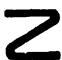
\includegraphics[keepaspectratio]{images/part002_84c4f053.jpg}}


\begin{enumerate}
\def\labelenumi{(\arabic{enumi})}
\setcounter{enumi}{4}
\tightlist
\item
任一素理想的幂不一定是准素理想（习题 1）。另一方面，存在不是素理想幂的准素理想（习题 1）。
\end{enumerate}

命题 2. 设 M 是诺特环上的模，p 是 A 的素理想，\((Q_{i})_{i\in I}\) 是 M 的非空有限子模族，且这些子模关于 M 都是 p-准素的。则 \(\bigcap_{i\in I} Q_{i}\) 关于 M 是 p-准素的。

\(\mathrm{M}/\left(\bigcap_{i\in\mathrm{I}}\mathrm{Q}_{i}\right)\) 同构于一个 \(\neq0\) 的子模，它是直和 \(\bigoplus_{i\in\mathrm{I}}(\mathrm{M}/\mathrm{Q}_{i})\) 的子模。现在

\[
\operatorname{Ass} \left(\bigoplus_ {i \in I} (M / Q _ {i})\right) = \bigcup_ {i \in I} \operatorname{Ass} (M / Q _ {i}) = \{p \}
\]

（§ 1，第 1 节，命题 3 的推论 1）。因此 \(\operatorname{Ass}\left(M / \left(\bigcap_{i \in I} Q_i\right)\right) = \{p\}\)（§ 1，第 1 节，命题 3 及命题 2 的推论 1）。

命题 3. 设 A 是诺特环，S 是 A 的乘性子集，p 是 A 的素理想，M 是 A-模，N 是 M 的子模，且 \(i = i_{A}^{S}\) 是从 M 到 \(S^{-1}M\) 的典范映射。

\begin{enumerate}
\def\labelenumi{(\roman{enumi})}
\item
  假设 \(\mathfrak{p} \cap \mathbf{S} \neq \varnothing\)。若 \(\mathbf{N}\) 关于 \(\mathfrak{p}\) 是 \(\mathbf{M}\)-准素的，则 \(\mathbf{S}^{-1}\mathbf{N} = \mathbf{S}^{-1}\mathbf{M}\)。
\item
  假设 \(\mathfrak{p} \cap \mathbf{S} = \varnothing\)。要使 \(\mathbf{N}\) 关于 \(\mathfrak{p}\) 是 \(\mathbf{M}\)-准素的，充要条件是 \(\mathbf{N}\) 具有 \(i^{-1}(\mathbf{N}')\) 的形式，其中 \(\mathbf{N}'\) 是 \(\mathbf{S}^{-1}\mathbf{A}\)-子模，且是 \(\mathbf{S}^{-1}\mathbf{M}\) 的子模，并且关于 \((\mathbf{S}^{-1}\mathfrak{p})\) 是 \(\mathbf{S}^{-1}\mathbf{M}\)-准素的；此时 \(\mathbf{N}' = \mathbf{S}^{-1}\mathbf{N}\)。
\item
  如果 \(\mathfrak{p} \cap S \neq \varnothing\)，且 \(N\) 关于 \(\mathfrak{p}\) 是 \(M\)-准素的，则
\end{enumerate}

\[
\mathrm{Ass} _ {\mathbf {S} ^ {- 1} \mathbf {A}} (\mathrm{S} ^ {- 1} (\mathrm{M} / \mathrm{N})) = \varnothing
\]

（§ 1，第 2 节，命题 5 的推论），因此 \(S^{-1}(M/N) = 0\)（§ 1，第 1 节，命题 2 的推论 1），从而 \(S^{-1}M/S^{-1}N = 0\)。

\begin{enumerate}
\def\labelenumi{(\roman{enumi})}
\setcounter{enumi}{1}
\tightlist
\item
   假设\(\mathfrak{p} \cap \mathrm{S} = \varnothing\)。若\(\mathbf{N}\)是\(\mathfrak{p}\)-准素的（相对于\(\mathbf{M}\)），则\(\operatorname{Ass}_{\mathbf{S}^{-1}\mathbf{A}}(\mathrm{S}^{-1}(\mathrm{M/N})) = \{\mathrm{S}^{-1}\mathfrak{p}\}\)（\(\S 1\)，第 2 节，命题 5 的推论）因此，子模\(\mathbf{N}' = \mathrm{S}^{-1}\mathbf{N}\)的\(\mathrm{S}^{-1}\mathbf{M}\)是\((\mathrm{S}^{-1}\mathfrak{p})\)-准素的；此外，若\(s \in \mathbf{S}\)和\(m \in \mathbf{M}\)满足\(sm \in \mathbf{N}\)，则\(m \in \mathbf{N}\)，因为在\(s\)中比为\(\mathbf{M/N}\)的伸缩映射是单射，从而\(\mathbf{N} = \overline{i}^{1}(\mathbf{N}')\)（第二章，\(\S 2\)，第 4 节，命题 10）。反之，设\(\mathbf{N}'\)是\(\mathrm{S}^{-1}\mathbf{M}\)的子模，它是\((\mathrm{S}^{-1}\mathfrak{p})\)-准素的（相对于\(\mathrm{S}^{-1}\mathbf{M}\)）；记\(\mathbf{N} = \overline{i}^{1}(\mathbf{N}')\)；则\(\mathbf{N}' = \mathrm{S}^{-1}\mathbf{N}\)（第二章，\(\S 2\)，第 4 节，命题 10），并且\(\operatorname{Ass}_{\mathbf{S}^{-1}\mathbf{A}}(\mathrm{S}^{-1}(\mathrm{M/N})) = \operatorname{Ass}_{\mathbf{S}^{-1}\mathbf{A}}((\mathrm{S}^{-1}\mathbf{M})/\mathrm{N}') = \{\mathrm{S}^{-1}\mathfrak{p}\}\)。由于典范映射\(\mathrm{M/N} \to \mathrm{S}^{-1}(\mathrm{M/N})\)是单射，\(\mathbf{A}\)中与\(\mathbf{M/N}\)相关联的每个素理想都不与\(\mathbf{S}\)相交（\(\S 1\)，第 2 节，命题 6）；因此\(\operatorname{Ass}(\mathrm{M/N}) = \{\mathfrak{p}\}\)（\(\S 1\)，第 2 节，命题 5 的推论），所以\(\mathbf{N}\)是\(\mathfrak{p}\)-准素的（相对于\(\mathbf{M}\)）。
\end{enumerate}

\subsection{准素分解的存在性}

定义 2. 设 A 是诺特环，M 是 A-模，N 是 M 的子模。M 的一族有限个关于 M 为准素的子模 \((\mathbf{Q}_i)_{i\in I}\)，若满足 \(\mathbf{N} = \bigcap_{i\in I}\mathbf{Q}_i\)，则称为 N 在 M 中的准素分解。

例。取 \(\mathbf{A} = \mathbf{Z}\)，\(\mathbf{M} = \mathbf{Z}\)，\(\mathbf{N} = n\mathbf{Z}\)，其中整数 \(n > 0\)。若 \(n = p_{1}^{\alpha_1} \ldots p_{k}^{\alpha_k}\) 是 \(n\) 的素因子分解，

\[
n \mathbf {Z} = (p _ {1} ^ {\alpha_ {1}} \mathbf {Z}) \cap \dots \cap (p _ {k} ^ {\alpha_ {k}} \mathbf {Z})
\]

这是 \(n\mathbf{Z}\) 在 \(\mathbf{Z}\) 中的准素分解，由第 1 节例 4 得出。

滥用语言地说，关系\(\mathbf{N} = \bigcap_{i \in I} \mathbf{Q}_i\)称为\(\mathbf{N}\)中的准素分解\(\mathbf{M}\)。同样也可说，\(\{0\} = \bigcap_{i \in I} (\mathbf{Q}_i / \mathbf{N})\)是\(\{0\}\)中的准素分解\(\mathbf{M} / \mathbf{N}\)。如果\((\mathbf{Q}_i)_{i \in I}\)是\(\mathbf{N}\)中的准素分解\(\mathbf{M}\)，典范映射从\(\mathbf{M} / \mathbf{N}\)到\(\bigoplus_{i \in I} (\mathbf{M} / \mathbf{Q}_i)\)是单射。反之，设\(\mathbf{N}\)是\(\mathbf{M}\)的子模，且\(f\)是从\(\mathbf{M} / \mathbf{N}\)到有限直和\(\mathbf{P} = \bigoplus_{i \in I} \mathbf{P}_i\)，其中每个集合\(\operatorname{Ass}(\mathbf{P}_i)\)都归结为单个元素\(p_i\)；令\(f_i\)是同态\(\mathbf{M} / \mathbf{N} \to \mathbf{P}_i\)，它由\(f\)与投影\(\mathbf{P} \to \mathbf{P}_i\)的复合得到，并令\(Q_i / \mathbf{N}\)是\(f_i\)的核；则与\(Q_i\)不同的\(\mathbf{M}\)关于\(\mathbf{M}\)都是准素的（第 1 节，定义 1），且\(\mathbf{N} = \bigcap_{i \in I} Q_i\)。此外，\(\operatorname{Ass}(\mathbf{M} / \mathbf{N}) \subset \bigcup_{i \in I} \{\mathfrak{p}_i\}\)（根据第 1 节，第 1 节，命题 3 的推论 2）。

定理 1. 设 M 是诺特环上的有限生成模，N 是 M 的子模。存在如下形式的 N 的准素分解

\[
N = \bigcap_ {\mathfrak {p} \in \operatorname{Ass} (M / N)} Q (\mathfrak {p})\tag{1}
\]

其中，对于所有 \(\mathfrak{p} \in \operatorname{Ass}(\mathbf{M} / \mathbf{N})\)，\(\mathbf{Q}(\mathfrak{p})\) 是 \(\mathfrak{p}\)-准素的（相对于 \(\mathbf{M}\)）。

我们可以用 M/N 替换 M，因而设 N = 0。根据 § 1，第 4 节，定理 2 的推论，Ass(M) 是有限集；根据 § 1，第 1 节，命题 4，对于每个 \(p \in \text{Ass}(M)\)，存在 M 的一个子模 \(Q(p)\)，使得 \(\text{Ass}(M/Q(p)) = \{p\}\) 且 \(\text{Ass}(Q(p)) = \text{Ass}(M) - \{p\}\)。记 \(P = \bigcap_{p \in \text{Ass}(M)} Q(p)\)；对于所有 \(p \in \text{Ass}(M)\)，有 \(\text{Ass}(P) \subset \text{Ass}(Q(p))\)，从而 \(\text{Ass}(P) = \varnothing\)，这意味着 P = 0（§ 1，第 1 节，命题 2 的推论 1），因而定理得证。

\subsection{准素分解的唯一性性质}

定义 3. 设 M 是诺特环上的模，N 是 M 的子模。M 中 N 的准素分解 \(N = \bigcap_{i \in I} Q_i\) 称为既约的，如果满足下列条件：

\begin{enumerate}
\def\labelenumi{(\alph{enumi})}
\item
  不存在指标 \(i \in \mathbf{I}\)，使得 \(\bigcap_{j \neq i} Q_j \subset Q_i\)；
\item
  若 \(\operatorname{Ass}(\mathbf{M} / \mathbf{Q}_i) = \{\mathfrak{p}_i\}\)，则 \(\mathfrak{p}_i\)（\(i \in \mathbf{I}\)）彼此不同。
\end{enumerate}

从\(\mathbf{N} = \bigcap_{i\in \mathbf{I}}\mathbf{Q}_i\)在\(\mathbf{N}\)中的\(\mathbf{M}\)中可以如下导出\(\mathbf{M}\)在\(\mathbf{N}\)中：令\(\mathbf{J}\)为\(\mathbf{I}'\)的子集所成集合中满足\(\mathbf{I}\)使得\(\mathbf{N} = \bigcap_{i\in \mathbf{I}'}\mathbf{Q}_i\)。显然，\((\mathbf{Q}_i)_{i\in \mathbf{J}}\)满足条件 (a)。再令\(\Phi\)为由\(p_i\)组成且满足\(i\in J\)；对于所有\(p\in \Phi\)，令\(H(p)\)为由\(i\in J\)组成且满足\(p_i = p\)，并令\(Q(p) = \bigcap_{i\in H(p)}Q_i\)；由第 1 节命题 2 可知，\(Q(p)\)是\(p\)-准素的（相对于\(M\)）；此外\(N = \bigcap_{p\in \Phi}Q(p)\)，所以族\(Q((p))_{p\in \Phi}\)从而是\(N\)在\(M\)中的既约准素分解。我们将看到，第 2 节定理 1 的证明中定义的准素分解是既约的；这由下述命题推出：

命题 4. 设 M 是诺特环上的模，N 是 M 的子模，\(N = \bigcap_{i \in I} Q_i\) 是 N 在 M 中的准素分解；对于所有 \(i \in I\)，令 \(\{p_i\} = \text{Ass}(M/Q_i)\)。该分解为既约的充要条件是：各 \(p_i\) 彼此不同且属于 \(\text{Ass}(M/N)\)；此时

\begin{enumerate}
\def\labelenumi{(\arabic{enumi})}
\setcounter{enumi}{1}
\tightlist
\item
\end{enumerate}

\[
\operatorname{Ass} (\mathbf {M} / \mathbf {N}) = \bigcup_ {i \in I} \left\{\mathfrak {p} _ {i} \right\}\tag{3}
\]

\[
\operatorname{Ass} \left(\mathrm{Q} _ {i} / \mathrm{N}\right) = \bigcup_ {j \neq i} \left\{\mathfrak {p} _ {j} \right\} \quad \text{对所有 } i \in \mathrm{I}.
\]

若陈述中的条件满足，\(N = \bigcap_{j \neq i} Q_j\)不可能成立，因为否则可推出\(\text{Ass}(M/N) \subset \bigcup_{j \neq i} \{p_j\}\)（§ 1，第 1 节，命题 3 的推论 2），这与假设矛盾；于是 N 的准素分解\((Q_i)_{i \in I}\)必然是既约的。反之，\(\text{Ass}(M/N) \subset \bigcup_{i \in I} \{p_i\}\)总是成立（§ 1，第 1 节，命题 3 的推论 2）；另一方面，对所有\(i \in I\)，令\(P_i = \bigcap_{j \neq i} Q_j\)；则\(P_i \cap Q_i = N\)，且若\(P_i \neq N\)是既约的，则\((Q_i)_{i \in I}\)非零，并同构于子模\(P_i/N\)中的\((P_i + Q_i)/Q_i\)，从而\(M/Q_i\)（§ 1，第 1 节，命题 3 及命题 2 的推论 1）；由于\(\{p_i\} = \text{Ass}(P_i/N)\)，\(P_i/N \subset M/N\)，\(p_i \in \text{Ass}(M/N)\)这就完成了陈述中条件之必要性的证明以及公式 (2) 的证明。最后，由于\(N = \bigcap_{j \neq i} (Q_j \cap Q_i)\)，\(\text{Ass}(Q_i/N) \subset \bigcup_{j \neq i} \text{Ass}(Q_i/(Q_j \cap Q_i))\)（§ 1，第 1 节，命题 3 的推论 2）；但\(Q_i/(Q_j \cap Q_i)\)同构于子模\((Q_i + Q_j)/Q_j\)中的\(M/Q_j\)，故\(\text{Ass}(Q_i/(Q_j \cap Q_i)) \subset \{p_j\}\)，且并且

\[
\operatorname{Ass} \left(Q _ {i} / N\right) \subset \bigcup_ {j \neq i} \left\{\mathfrak {p} _ {j} \right\};
\]

计及 (2) 及 §1 第 1 节的命题 3，公式 (3) 即易得。

推论。设 A 是诺特环，M 是 A-模，N 是 M 的子模，且 \((\mathbf{Q}_{i})_{i\in I}\) 是 N 在 M 中的准素分解。则 \(\operatorname{Card}(\mathbf{I}) \geqslant \operatorname{Card}(\operatorname{Ass}(\mathbf{M}/\mathbf{N}))\)；要使 \((\mathbf{Q}_{i})_{i\in I}\) 成为既约准素分解，充要条件是 \(\operatorname{Card}(\mathbf{I}) = \operatorname{Card}(\operatorname{Ass}(\mathbf{M}/\mathbf{N}))\)。

由命题 4 前的说明可知，存在 \((\mathbf{R}_j)_{j\in J}\) 作为 \(N\) 在 \(M\) 中的既约准素分解，使得 \(\operatorname{Card}(J) \leqslant \operatorname{Card}(I)\)；第一个断言于是由第二个断言得出，而后者是命题 4 的结果。

命题 5. 设 A 是诺特环，M 是 A-模，N 是 M 的子模，\(\mathbf{N} = \bigcap_{i \in I} \mathbf{Q}_i\) 是 N 在 M 中的既约准素分解；对于所有 \(i \in I\)，令 \(\{\mathfrak{p}_i\} = \operatorname{Ass}(\mathbf{M} / \mathbf{Q}_i)\)。若 \(\mathfrak{p}_i\) 是 \(\operatorname{Ass}(\mathbf{M} / \mathbf{N})\) 的极小元，则 \(\mathbf{Q}_i\) 等于 N 关于 \(\mathfrak{p}_i\) 的饱和（第二章，第 2 节，第 4 节）（参见习题 2）。

显然可以只考虑 N = 0 的情形，必要时以 M/N 替换 M。若 \(p_{i}\) 是 Ass(M) 中的极小元，则 Ass(M) 中不与 A - \(p_{i}\) 相交的元素所成的集合归结为 \(p_{i}\)；命题于是由上面的公式 (3) 以及 §1，第 2 节，命题 6 得出，因为典范映射 \(M \to M_{p_{i}}\) 的核等于关于 \(p_{i}\) 的 0 的饱和（第二章，第 2 节，第 4 节）。

注。属于\(\mathfrak{p}_i\in\mathrm{Ass}(\mathbf{M}/\mathbf{N})\)的素理想，如果不是该集合的极小元，有时称为与\(\mathbf{M}/\mathbf{N}\)相伴的浸入素理想；若\(\mathbf{M}/\mathbf{N}\)是有限生成的，则对于\(\mathfrak{p}_0\in\mathrm{Ass}(\mathbf{M}/\mathbf{N})\)成为浸入素理想的充要条件是\(\mathrm{V}(\mathfrak{p}_0)\)不是\(\mathrm{Supp}(\mathbf{M}/\mathbf{N})\)的不可约分支（第二章，第 4 节，第 3 节，命题 14 的推论 2）；若\((\mathrm{Q}(\mathfrak{p}))_{\mathfrak{p}\in\mathrm{Ass}(\mathbf{M}/\mathbf{N})}\)和\((\mathrm{Q}'(\mathfrak{p}))_{\mathfrak{p}\in\mathrm{Ass}(\mathbf{M}/\mathbf{N})}\)是\(\mathbf{N}\)在\(\mathbf{M}\)中的两个既约准素分解，则可能有\(\mathrm{Q}'(\mathfrak{p}_0)\neq\mathrm{Q}(\mathfrak{p}_0)\)（习题 24 (c)）；总可以通过对其中出现的准素子模附加补充条件，定义\(\mathbf{N}\)在\(\mathbf{M}\)中的典范既约准素分解（习题 4）。

\subsection{准素分解的局部化}

给定诺特环 A 上模 M 的一个子模 N，为简便起见，本节将 \(D_{I}(M/N)\) 记为 N 在 M 中的、索引集为 I（与 Ass(M/N) 等势）的既约准素分解所成的集合。

命题 6. 设 A 是诺特环，M 是 A-模，N 是 M 的子模，且 I = Ass(M/N)。设 S 是 A 的乘性子集，J 是 I 的子集，由指标 \(i\) 组成，且这些指标满足 \(\mathbf{S} \cap \mathfrak{p}_i = \varnothing\)。令 \(\mathbf{N}'\) 是 \(\mathbf{N}\) 关于 \(\mathbf{S}\) 在 \(\mathbf{M}\) 中的饱和。则：

\begin{enumerate}
\def\labelenumi{(\roman{enumi})}
\item
  如果 \((\mathbf{Q}_i)_{i\in I}\) 是 \(\mathbf{D}_{\mathrm{I}}(\mathbf{M} / \mathbf{N})\) 的元素，则族 \((\mathbf{Q}_i)_{i\in J}\) 是 \(\mathbf{D}_{J}(\mathbf{M} / \mathbf{N}')\) 的元素，且族 \((\mathbf{S}^{-1}\mathbf{Q}_i)_{i\in J}\) 是 \(\mathbf{D}_{J}(\mathbf{S}^{-1}\mathbf{M} / \mathbf{S}^{-1}\mathbf{N})\) 的元素。
\item
  映射 \((\mathbf{Q}_i)_{i\in J}\to (\mathbf{S}^{-1}\mathbf{Q}_i)_{i\in J}\) 是从 \(\mathrm{D}_{\mathrm{J}}(\mathbf{M} / \mathbf{N}^{\prime})\) 到 \(\mathbf{D}_{\mathrm{J}}(\mathbf{S}^{-1}\mathbf{M} / \mathbf{S}^{-1}\mathbf{N})\) 的双射。
\item
   如果\((\mathbf{Q}_i)_{i\in J}\)是\(\mathbf{D}_{\mathbf{J}}(\mathbf{M} / \mathbf{N}')\)的元素，而\((\mathbf{R}_i)_{i\in I}\)是\(\mathbf{D}_{\mathbf{I}}(\mathbf{M} / \mathbf{N})\)的元素，族\((\mathrm{T}_i)_{i\in I}\)满足\(\mathrm{T}_i = \mathrm{Q}_i\)对于\(i\in \mathbf{J}\)，且\(\mathrm{T}_i = \mathrm{R}_i\)对于\(i\in \mathbf{I} - \mathbf{J}\)的元素\(\mathbf{D}_{\mathbf{I}}(\mathbf{M} / \mathbf{N})\)。
\item
   我们知道（第 1 节，命题 3），对于\(i \in J\)，\(S^{-1}Q_{i}\)是关于\(S^{-1}p_{i}\)的准素子模，并且对于\(i \in I - J\)，\(S^{-1}Q_{i} = S^{-1}M\)；由于\(S^{-1}N = \bigcap_{i \in I} S^{-1}Q_{i}\)（第二章，第 2 节，第 4 节），所以也有\(S^{-1}N = \bigcap_{i \in J} S^{-1}Q_{i}\)。对于\(S^{-1}p_{i}\)，\(i \in J\)彼此不同，且其集合是\(\operatorname{Ass}(S^{-1}M / S^{-1}N)\)（§ 1，第 2 节，命题 5 的推论）；于是（命题 4），\(S^{-1}Q_{i})_{i \in J}\)是\(S^{-1}N\)的既约准素分解。此外，\(Q_{i} = (i_{M}^{S})^{-1}(S^{-1}Q_{i})\)（第 1 节命题 3），所以\(N' = (i_{M}^{S})^{-1}(S^{-1}N) = \bigcap_{i \in J} Q_{i}\)，而\((Q_{i})_{i \in J}\)显然是\(N'\)中的既约准素分解。
\item
   由于\(S^{-1}N' = S^{-1}N\)，我们可以用\(N'\)替换 N，即设 J = I。令\((P_i)_{i \in I}\)是\(S^{-1}N\)在\(S^{-1}M\)中的既约准素分解，并记\(Q_i = (i_M^S)^{-1}(P_i)\)；根据第 1 节命题 3，\(Q_i\)是关于\(p_i (i \in I)\)的准素子模，并且\((Q_i)_{i \in I}\)随后是 N 在 M 中的既约准素分解。最后，对所有\(i \in I\)以及 M 的每个子模\(Q'_i\)，若 M 关于\(p_i\)-准素，则\(Q'_i = (i_M^S)^{-1}(S^{-1}Q'_i)\)（根据第 1 节命题 3），我们定义了两个映射\(D_I(M/N) \to D_I(S^{-1}M/S^{-1}N)\)和\(D_I(S^{-1}M/S^{-1}N) \to D_I(M/N)\)，它们的复合分别是\(D_I(M/N)\)和\(D_I(S^{-1}M/S^{-1}N)\)上的恒等映射，这就证明了 (ii)。
\item
  根据 (i)，\(\mathbf{N}' = \bigcap_{i\in J}\mathbb{R}_i\)，从而
\end{enumerate}

\[
\mathrm{N} = \mathrm{N} ^ {\prime} \cap \bigcap_ {i \in \mathrm{I} - J} \mathrm{R} _ {i} = \left(\bigcap_ {i \in J} \mathrm{Q} _ {i}\right) \cap \left(\bigcap_ {i \in \mathrm{I} - J} \mathrm{R} _ {i}\right)
\]

并且由第 3 节命题 4 的推论立即可知该准素分解是既约的。

推论。映射

\[
\mathrm{D} _ {\mathrm{I}} (\mathrm{M} / \mathrm{N}) \rightarrow \mathrm{D} _ {\mathrm{J}} (\mathrm{M} / \mathrm{N} ^ {\prime}) \quad \text{且} \quad \mathrm{D} _ {\mathrm{I}} (\mathrm{M} / \mathrm{N}) \rightarrow \mathrm{D} _ {\mathrm{J}} (\mathrm{S} ^ {- 1} \mathrm{M} / \mathrm{S} ^ {- 1} \mathrm{N})
\]

在命题 6 (i) 中定义的映射是满射。

命题 6 (iii) 表明映射 \(\mathrm{D}_{\mathrm{I}}(\mathrm{M}/\mathrm{N}) \rightarrow \mathrm{D}_{\mathrm{J}}(\mathrm{M}/\mathrm{N}')\) 是满射，而命题 6 (ii) 随即表明映射

\[
\mathrm{D} _ {\mathrm{I}} (\mathrm{M} / \mathrm{N}) \rightarrow \mathrm{D} _ {\mathrm{J}} (\mathrm{S} ^ {- 1} \mathrm{M} / \mathrm{S} ^ {- 1} \mathrm{N})
\]

是满射。

\subsection{有限长度的环与模}

若 A-模 M 具有有限长度，我们将此长度记为 \(\text{long}_{\mathbf{A}}(\mathbf{M})\) 或 \(\text{long}(\mathbf{M})\)。回忆，每个 Artin 环都是诺特环（代数，第八章，第 6 节，第 5 节，命题 12 的推论 3），每个 Artin 环上的有限生成模都具有有限长度（同上，命题 12 的推论 1）。此外，每个 Artin 整环都是域（代数，第八章，第 6 节，第 4 节，命题 9）。

命题 7. 设 M 是诺特环 A 上的有限生成模。下列性质等价：

\begin{enumerate}
\def\labelenumi{(\alph{enumi})}
\item
  M 具有有限长度。
\item
  每个理想 \(\mathfrak{p} \in \operatorname{Ass}(\mathbf{M})\) 都是 \(\mathbf{A}\) 的极大理想。
\item
  每个理想 \(\mathfrak{p} \in \operatorname{Supp}(\mathbf{M})\) 都是 \(\mathbf{A}\) 的极大理想。
\end{enumerate}

令 \((\mathbf{M}_i)_{0\leqslant i\leqslant n}\) 是 M 的一个合成列，使得对于 \(0\leqslant i\leqslant n - 1\)，\(\mathbf{M}_i / \mathbf{M}_{i + 1}\) 同构于 \(\mathrm{A} / \mathfrak{p}_i\)，其中 \(\mathfrak{p}_i\) 是素理想（§ 1，第 4 节，定理 1）。若 M 具有有限长度，则每个 A-模 \(\mathrm{A} / \mathfrak{p}_i\) 也具有有限长度，这意味着每个环 \(\mathrm{A} / \mathfrak{p}_i\) 都是 Artin 环；但由于 \(\mathrm{A} / \mathfrak{p}_i\) 是整环，故它是域，换言之 \(\mathfrak{p}_i\) 是极大理想；由此 (a) 蕴含 (b)（§ 1，第 4 节，定理 2）。条件 (b) 由 § 1，第 3 节，命题 7 蕴含 (c)。最后，若 \(\operatorname {Supp}(\mathbf{M})\) 中的所有理想都是极大理想，则 \(\mathfrak{p}_i\) 也都是极大理想（§ 1，第 4 节，定理 2），于是 \(\mathrm{A} / \mathfrak{p}_i\) 是单 A-模，M 具有有限长度，证明完成。

推论 1. 对于诺特环 A 上的每个有限长度模 M，都有 \(\operatorname{Ass}(\mathbf{M}) = \operatorname{Supp}(\mathbf{M})\)。

此时 \(\operatorname{Supp}(\mathbf{M})\) 的每个元素都是 \(\operatorname{Supp}(\mathbf{M})\) 的极小元，结论由 § 1，第 3 节，命题 7 的推论 1 得出。

推论 2. 设 M 是诺特环 A 上的有限生成模，p 是 A 的素理想。要使 \(M_{p}\) 成为非零的有限长度 \(A_{p}\)-模，充要条件是 p 为 Ass(M) 的极小元。

根据 § 1，第 2 节，命题 5 的推论，\(\operatorname{Ass}_{\mathbf{A}_{\mathfrak{p}}}(\mathbf{M}_{\mathfrak{p}})\)是理想\(q_{\mathfrak{p}}\)所成的集合，其中\(q\)遍历\(\operatorname{Ass}(\mathbf{M})\)中包含于\(p\)。（第二章，第 4 节，第 4 节），另一方面，\(p_{\mathfrak{p}}\)是\(\mathbf{A}_{\mathfrak{p}}\)的唯一极大理想；根据命题 7，要使\(\mathbf{M}_{\mathfrak{p}}\)成为\(\mathbf{A}_{\mathfrak{p}}\)的有限长度模，充要条件是没有属于\(\operatorname{Ass}(\mathbf{M})\)的元素严格包含于\(p\)。另一方面，对于\(\mathbf{M}_{\mathfrak{p}} \neq 0\)，根据定义，充要条件是\(\mathfrak{p} \in \operatorname{Supp}(\mathbf{M})\)（第二章，第 4 节，第 4 节），也就是说\(\mathfrak{p}\)包含\(\operatorname{Ass}(\mathbf{M})\)中的一个元素（§ 1，第 3 节，命题 7 的推论）。推论得证。

注 (1)。设 M 是诺特环 A 上的有限生成模；令\((\mathbf{M}_{i})_{0\leqslant i\leqslant n}\)是 M 的合成列，使得对于\(0\leqslant i\leqslant n-1\)，\(M_{i}/M_{i+1}\)同构于\(A/p_{i}\)，其中\(p_{i}\)是 A 的素理想（§ 1，第 4 节，定理 1）。若 p 是 Ass(M) 的极小元，则长度\(\text{long}_{A_{p}}(M_{p})\)等于满足\(p_{i}=p\)的指标 i 的数目。因为\((\mathbf{M}_{i})_{p}\)构成\(M_{p}\)的合成列，且\((\mathbf{M}_{i})_{p}/(\mathbf{M}_{i+1})_{p}\)同构于\((\mathbf{A}/p_{i})_{p}\)并且因此同构于\(\{0\}\)，当\(p_{i}\neq p\)（因为根据 § 1，第 4 节，定理 2，p 是\(p_{i}\)所成集合中的极小元）并且同构于\((\mathbf{A}/p)_{p}\)是一个域，当\(p_{i}=p\)时。

命题 8. 设 M 是诺特环上的有限长度模。

\begin{enumerate}
\def\labelenumi{(\roman{enumi})}
\item
  以\(\{0\}\)为关于\(\mathbf{M}\)、以\(\operatorname{Ass}(\mathbf{M})\)（必然是既约的）；令\(\{0\} = \bigcap_{\mathfrak{p} \in \operatorname{Ass}(\mathbf{M})} \mathbf{Q}(\mathfrak{p})\)为此分解，其中\(\mathbf{Q}(\mathfrak{p})\)是\(\mathfrak{p}\)准素的（相对于\(\mathbf{M}\)）。
\item
  存在整数 \(n_0\)，使得对于所有 \(n \geqslant n_0\) 及所有 \(\mathfrak{p} \in \operatorname{Ass}(\mathbf{M})\)，都有 \(\mathbf{Q}(\mathfrak{p}) = \mathfrak{p}^n\mathbf{M}\)。
\item
  对于所有 \(\mathfrak{p} \in \operatorname{Ass}(\mathbf{M})\)，从 \(\mathbf{M}\) 到 \(\mathbf{M}_{\mathfrak{p}}\) 的典范映射是满射，且其核为 \(\mathbf{Q}(\mathfrak{p})\)。
\item
  从 \(\mathbf{M}\) 到 \(\bigoplus_{\mathfrak{p} \in \mathbf{Ass}(\mathbf{M})} (\mathbf{M} / \mathbf{Q}(\mathfrak{p}))\) 的典范单射是双射。
\end{enumerate}

由于每个元素\(\mathfrak{p} \in \operatorname{Ass}(M)\)都是\(\operatorname{Ass}(M)\)（命题 7），断言 (i) 由第 3 节命题 5 得出。由于\(M\)是有限生成的，存在\(n_0\)，使得\(\mathfrak{p}^n M \subset Q(\mathfrak{p})\)对于所有\(\mathfrak{p} \in \operatorname{Ass}(M)\)以及所有\(n \geqslant n_0\)（第 1 节，注）；但由于\(\mathfrak{p}\)是极大理想，\(\mathfrak{p}^n M\)是\(\mathfrak{p}\)-准素的（相对于\(M\)）（第 1 节，例 2 和例 3）；又由于\(\bigcap_{\mathfrak{p} \in \operatorname{Ass}(M)} \mathfrak{p}^n M = \{0\}\)，由 (i) 必然有\(\mathfrak{p}^n M = Q(\mathfrak{p})\)对于所有\(\mathfrak{p} \in \operatorname{Ass}(M)\)；从而得到 (ii)。由于\(\mathfrak{p}^n\)对于\(\mathfrak{p} \in \operatorname{Ass}(M)\)彼此互素，典范映射\(M \to \bigoplus_{\mathfrak{p} \in \operatorname{Ass}(M)} (M / \mathfrak{p}^n M)\)是满射（第二章，第 1 节，第 2 节，命题 6），从而得到 (iv)。于是\(\operatorname{Ass}(Q(\mathfrak{p})) = \operatorname{Ass}(M) - \{\mathfrak{p}\}\)以及\(\operatorname{Ass}(M / Q(\mathfrak{p})) = \{\mathfrak{p}\}\)（第 3 节，命题 4）；由于\(\operatorname{Ass}(M)\)的元素都是极大理想，\(\mathfrak{p}\)是\(\operatorname{Ass}(M)\)中唯一不与\(A - \mathfrak{p}\)相交的元素；\(Q(\mathfrak{p})\)因而是典范映射\(j: M \to M_{\mathfrak{p}}\)的核（§ 1，第 2 节，命题 6）。若\(s \in A - \mathfrak{p}\)上的伸缩映射比值为\(M / Q(\mathfrak{p})\)的\(s\)伸缩映射根据关系\(\operatorname{Ass}(M / Q(\mathfrak{p})) = \{\mathfrak{p}\}\)（第 1 节，命题 1）是单射；由于\(M / Q(\mathfrak{p})\)是 Artin 模，该伸缩映射是双射（代数，第八章，第 1 节，第 2 节，引理 3）。典范映射\(M \to M / Q(\mathfrak{p})\)可写成\(f \circ j\)，其中\(f: M_{\mathfrak{p}} \to M / Q(\mathfrak{p})\)是 A-同态（第二章，第 2 节，第 2 节，命题 3）；由于\(\operatorname{Ker}(j) = \operatorname{Ker}(f \circ j) = Q(\mathfrak{p})\)，\(f\)是单射；我们得出\(j\)是满射且\(f\)是双射。

推论。若 M 是诺特环上具有有限长度的模，则

\[
\operatorname{long} _ {\mathbf {A}} (\mathbf {M}) = \sum_ {\mathfrak {p} \in \mathbf {A s s} (\mathbf {M})} \operatorname{long} _ {\mathbf {A p}} (\mathbf {M} _ {\mathfrak {p}}).\tag{4}
\]

这将由命题 8 (iv) 得出，只要我们证明

\[
\operatorname{long} _ {\mathbf {A}} (\mathbf {M} / \mathbf {Q} (\mathfrak {p})) = \operatorname{long} _ {\mathbf {A} _ {\mathfrak {p}}} (\mathbf {M} _ {\mathfrak {p}}).
\]

现在，根据第 1 节命题 1，对于\(s \in \mathbf{A} - \mathfrak{p}\)，伸缩映射比为\(s\)作用于\(\mathrm{M} / \mathrm{Q}(\mathfrak{p})\)上是单射；因此，对每个\(s\)，作用于\(\mathbf{R}\)的子模\(\mathrm{M} / \mathrm{Q}(\mathfrak{p})\)上的伸缩映射也是单射；又因为\(\mathbf{R}\)是 Artin 模，该伸缩映射是双射（代数，第八章，第 2 节，第 2 节，引理 3）；我们得出，\(\mathbf{A}\)-子模中的\(\mathrm{M} / \mathrm{Q}(\mathfrak{p})\)正是双射\(f: \mathbf{M}_{\mathfrak{p}} \to \mathbf{M} / \mathbf{Q}(\mathfrak{p})\)的\(\mathbf{A}_{\mathfrak{p}}\)-子模\(\mathbf{M}_{\mathfrak{p}}\)的像（第二章，第 2 节，第 3 节），从而得到断言。

命题 9. 设 A 是诺特环。下列条件等价：

\begin{enumerate}
\def\labelenumi{(\alph{enumi})}
\item
  A 是 Artin 环。
\item
  \(\mathbf{A}\) 的所有素理想都是极大理想。
\item
  Ass(A) 的所有元素都是极大理想。
\end{enumerate}

若这些条件满足，A 只有有限个素理想，它们全是极大理想且与 A-模 A 相伴；此外，A 是半局部环，其 Jacobson 根是幂零的。

称 A 为 Artin 环等价于称 A 是有限长度的 A-模；因此由命题 7，(a) 和 (c) 等价。显然 (b) 蕴含 (c)。最后，(a) 蕴含 (b)，因为每个 Artin 整环都是域。因此，(a)、(b) 和 (c) 等价。

假设这些条件成立。由于 A 的每个素理想都属于 Supp(A)，而 Supp(A) 的每个元素都包含 Ass(A) 中的一个元素（§ 1，第 3 节，命题 7），由 (c) 得 Ass(A) 正是 A 的所有素理想的集合；于是 A 只有有限个素理想，它们全是极大理想并且与 A-模 A 相伴。这显然蕴含 A 是半局部环；最后，我们知道 Artin 环的 Jacobson 根是幂零的（代数，第八章，第 6 节，第 4 节，定理 3）。

注 (2)。诺特环 A 满足命题 9 的条件，意味着 A 的谱是有限且离散的，因而 \(\operatorname{Spec}(A)\) 的每个点都是闭点（第二章，第 4 节，第 3 节，命题 11 的推论 6）。反之，对于诺特环 A，\(\operatorname{Spec}(A)\) 的每个点都是闭点，意味着 A 的每个素理想都是极大理想（同上），所以这一条件等价于命题 9 的条件。

推论 1. 每个 Artin 环 A 都同构于有限个 Artin 局部环的直积。

由命题 9 以及命题 8 (iii) 和 (iv) 可知，若 \((\mathfrak{m}_i)_{1\leqslant i\leqslant n}\) 是 A 的极大理想族，则典范映射 \(\mathbf{A}\to \prod_{i}\mathbf{A}_{m_i}\) 是双射。

注 (3)。这个推论也可以由 \(\operatorname{Spec}(A)\) 是有限且离散的事实以及第二章，第 4 节，第 3 节，命题 15 得出。

推论 2. 设 A 是诺特环，m 是 A 的一个理想。下列条件等价：

\begin{enumerate}
\def\labelenumi{(\alph{enumi})}
\item
  A 是半局部环，且 m 是 A 的定义理想。
\item
  A 是带有 m-进拓扑的 Zariski 环，且 A/m 是 Artin 环。
\end{enumerate}

若 (a) 成立，则 A 是带有 m-进拓扑的 Zariski 环（第三章，第 3 节，第 3 节，例 3）；此外，由假设 m 包含 A 的 Jacobson 根 r 的某个幂，故 A 中每个包含 m 的素理想也包含 r（第二章，第 1 节，第 1 节，命题 1）；由于 r 是极大理想的有限交（同上），它因此是极大理想；命题 9 于是表明 A/m 是 Artin 环。反之，若 (b) 成立，则 A 的每个极大理想 p 都包含 A 的 Jacobson 根，因而包含 m（第三章，第 3 节，第 3 节，命题 6）；由于 A/m 是 Artin 环，理想 p/m 只有有限多个（命题 9），所以 A 只有有限个极大理想，这意味着它是半局部环。

推论 3. 设 A、A' 是两个环，h 是从 A 到 A' 的同态。假设 A 是半局部诺特环，且 A' 是有限生成的 A-模。则环 A' 是半局部诺特环；如果 m 是 A 的定义理想，则 mA' 是 A' 的定义理想。

我们知道 A' 是带有 mA'-进拓扑的 Zariski 环（第三章，第 3 节，第 3 节，命题 7）。由于 A/m 是 Artin 环（推论 2），而 A'/mA' 是有限生成的 (A/m)-模，所以 A'/mA' 是 Artin 环，从而 A' 是半局部环且 mA' 是 A' 的定义理想（推论 2）。

推论 4. 设 A 是完备的半局部诺特环，m 是 A 的定义理想，E 是有限生成的 A-模，\((\mathbf{F}_{n})\) 是 E 的子模的递减序列，且 \(\bigcap_{n} F_{n} = 0\)。则对于所有 p \textgreater{} 0，存在 n \textgreater{} 0，使得 \(F_{n} \subset m^{p}E\)。

由于 A 是 Zariski 环，E 是 Hausdorff 的，且 \(F_{n}\) 在 m-进拓扑下是闭的。另一方面，E 是完备的（第三章，第 2 节，第 12 节，命题 16 的推论 1）。最后，\(E/m^{p}E\) 是环 \(A/m^{p}\) 上的有限生成模，而该环是 Artin 环（推论 2）；于是 \(E/m^{p}E\) 是 Artin 的 \((A/m^{p})\)-模，因而也是 Artin 的 A-模。推论于是由第三章，第 2 节，第 7 节，命题 8 得出。

推论 5. 在完备的半局部诺特环中，交为 0 的每个递减理想序列都是收敛到 0 的滤子基。

只需将推论 4 应用于 A-模 A。

命题 10. 设 A 是诺特环，\(\mathfrak{p}_1, \ldots, \mathfrak{p}_n\) 是与 A-模 A 相伴的素理想，其中当 \(\mathfrak{p}_i \neq \mathfrak{p}_j\) 时 \(i \neq j\)。

\begin{enumerate}
\def\labelenumi{(\roman{enumi})}
\item
  集合 \(\mathbf{S} = \bigcap_{i=1}^{n} (\mathbf{A} - \mathfrak{p}_i)\) 是 A 中不是零因子的元素所成的集合。\\
\item
  如果所有 \(\mathfrak{p}_i\) 都是 \(\operatorname{Ass}(\mathbf{A})\) 的极小元，则 \(\mathbf{S}^{-1}\mathbf{A}\) 是 \(\mathbf{A}\) 的全分式环，并且是 Artin 环。
\item
  如果环 A 是约化的，则所有 \(p_{i}\) 都是 Ass(A) 的极小元（因而也是 Spec(A) 的极小元），且每个 \(A_{p_{i}}\) 都是域；对于每个指标 i，典范同态 \(S^{-1}A \to A_{p_{i}}\)（第二章，第 2 节，第 1 节，命题 2 的推论 1）是满射，且其核是 \(S^{-1}p_{i}\)；最后，从 \(S^{-1}A\) 到 \(\prod_{i=1}^{n} (S^{-1}A/S^{-1}p_{i})\) 的典范同态是双射。
\end{enumerate}

S 是 A 中不是零因子的元素所成的集合这一事实已经见于（\(\S\) 1，第 1 节，命题 2 的推论 3）。\(S^{-1}A\) 的素理想是

形如\(\mathbf{S}^{-1}\mathfrak{p}\)，其中\(\mathfrak{p}\)是\(\mathbf{A}\)的素理想，且包含于\(\bigcup_{i=1}^{n} \mathfrak{p}_i\)（第二章，第 2 节，第 5 节，命题 10），也就是包含于\(\mathfrak{p}_i\)（第二章，第 1 节，第 1 节，命题 2）。若\(\mathfrak{p}_i\)是\(\operatorname{Ass}(\mathbf{A})\)的极小元，则它是\(\operatorname{Spec}(\mathbf{A})\)的极小元（§ 1，第 3 节，命题 7 的推论）；若\(\mathfrak{p}_i\)是\(\operatorname{Ass}(\mathbf{A})\)，则可见\(\mathbf{S}^{-1}\mathbf{A}\)的素理想正是\(\mathbf{S}^{-1}\mathfrak{p}_i\)，因而它们全是极大理想，这就证明\(\mathbf{S}^{-1}\mathbf{A}\)是 Artin 环（命题 9）。

最后设环 A 是约化的。则 \(\bigcap_{i=1}^{n} p_i = \{0\}\)（§ 1，第 3 节，

命题 7 的推论 2）。我们推出\(\{0\} = \bigcap_{i=1}^{n} p_i\)是理想\(\{0\}\)的既约准素分解（第 3 节，命题 4 的推论）；特别地，没有一个\(p_i\)能包含指标为\(p_j\)的\(j \neq i\)，从而\(p_i\)都是\(\operatorname{Ass}(A)\)的极小元。根据 (ii)，环\(S^{-1}A\)是 Artin 环。\(S^{-1}p_i\)是与\(S^{-1}A\)-模\(S^{-1}A\)相伴的素理想（\(\S\)1，第 2 节，命题 5 的推论），并且\(\{0\} = S^{-1}\left(\bigcap_{i=1}^{n} p_i\right) = \bigcap_{i=1}^{n} S^{-1}p_i\)（第二章，\(\S\)2，第 4 节）；由于\(S^{-1}p_i\)彼此不同，\((S^{-1}p_i)_{1 \leqslant i \leqslant n}\)是\(\{0\}\)在\(S^{-1}A\)中的既约准素分解（第 3 节，命题 4 的推论）。命题 8 表明，典范同态\(g_{i} \colon S^{-1}\mathbf{A} \to (\mathbf{S}^{-1}\mathbf{A})_{p_{i}}\)是满射，且核为\(S^{-1}p_{i}\)；典范同态\(S^{-1}\mathbf{A} \to \prod_{i=1}^{n} (\mathbf{S}^{-1}\mathbf{A}/\mathbf{S}^{-1}p_{i})\)是双射。此外我们知道，典范同态\(S^{-1}\mathbf{A} \to A_{p_{i}}\)是由\(g_{i}\)与同构\((\mathbf{S}^{-1}\mathbf{A})_{\mathbf{S}^{-1}p_{i}} \to A_{p_{i}}\)的复合（第二章，第 2 节，第 3 节，命题 7）。最后，由命题 8，\((\mathbf{S}^{-1}\mathbf{A})_{\mathbf{S}^{-1}p_{i}}\)同构于\(S^{-1}\mathbf{A}/\mathbf{S}^{-1}p_{i}\)，因而是域，因为\(S^{-1}p_{i}\)是极大理想。

\subsection{准素分解与纯量扩张}

本节中，A 和 B 表示两个环；我们考虑环同态\(\rho: \mathbf{A} \to \mathbf{B}\)，它使 B 成为 A-代数；回忆，对于每个 B-模 F，\(\rho_*(\mathbf{F})\)是交换群 F，其 A-模结构由\(a.y = \rho(a)y\)对所有\(a \in \mathbf{A}, y \in \mathbf{F}\)定义。

引理 1. 设 A 是诺特环，p 是 A 的素理想，E 是 A-模，其湮灭子包含 p 的某个幂，且 \(\operatorname{Ass}(\mathbf{E}) = \{\mathfrak{p}\}\)；F 是 B-模，且 \(\rho_{*}(\mathbf{F})\) 是平坦的 A-模。则条件 \(\mathfrak{P} \in \operatorname{Ass}_{\mathbf{B}}(\mathbf{E} \otimes_{\mathbf{A}} \mathbf{F})\) 蕴含 \(\overline{\rho}^{1}(\mathfrak{P}) = \mathfrak{p}\)。

若\(n\)满足\(p^n\mathbf{E} = 0\)，则\(p^n\mathbf{B} \subset \operatorname{Ann}(\mathbf{E} \otimes_{\mathbf{A}} \mathbf{F})\)，从而\(p^n\mathbf{B} \subset \mathfrak{P}\)，这意味着\(p^n \subset \overline{\rho}^1(\mathfrak{P})\)，因而\(p \subset \overline{\rho}^1(\mathfrak{P})\)，因为\(\overline{\rho}^1(\mathfrak{P})\)是素理想。此外，若\(a \in \mathbf{A} - p\)，则\(h\)上的伸缩映射比为\(a\)，且在\(\mathbf{E}\)上是单射（§ 1，第 1 节，命题 2 的推论 2）；由于\(h \otimes l_{\mathbf{F}}\)是作用于\(h'\)的伸缩映射，其比为\(\rho(a)\)，作用于\(\mathbf{E} \otimes_{\mathbf{A}} \mathbf{F}\)上，且\(\rho_*(\mathbf{F})\)是平坦的，故\(h'\)是单射（第一章，第 2 节，第 2 节，定义 1）；这证明\(\rho(a) \notin \mathfrak{P}\)，从而\(\overline{\rho}^1(\mathfrak{P}) = p\)。

定理 2. 设 \(\rho: \mathbf{A} \to \mathbf{B}\) 是环同态，E 是 A-模，F 是 B-模，且 \(\rho_*(\mathbf{F})\) 是平坦的 A-模。则

\[
\operatorname{Ass} _ {\mathbf {B}} (\mathrm{E} \otimes_ {\mathbf {A}} \mathrm{F}) \supset \bigcup_ {\mathfrak {p} \in \operatorname{Ass} _ {\mathbf {A}} (\mathrm{E})} \operatorname{Ass} _ {\mathbf {B}} (\mathrm{F} / \mathfrak {p} \mathrm{F}).\tag{5}
\]

当 A 是诺特环时，(5) 两边相等。

令 \(\mathfrak{p} \in \operatorname{Ass}_{\mathbf{A}}(\mathbf{E})\)；根据定义，存在正合列

\[
0 \rightarrow \mathrm{A} / \mathfrak {p} \rightarrow \mathrm{E}.
\]

由于 F 是平坦的 A-模，我们得到正合列

\[
0 \rightarrow \mathrm{F} / \mathfrak {p} \mathrm{F} \rightarrow \mathrm{E} \otimes_ {\mathrm{A}} \mathrm{F}
\]

从而 \(\operatorname{Ass}_{\mathbf{B}}(\mathbf{F} / p\mathbf{F})\subset \operatorname{Ass}_{\mathbf{B}}(\mathbf{E}\otimes_{\mathbf{A}}\mathbf{F})\)，这就证明了包含关系 (5)。

现在假设 A 是诺特环，我们来证明反向包含关系。

我们分步进行：

\begin{enumerate}
\def\labelenumi{(\roman{enumi})}
\tightlist
\item
  首先假设 E 是有限生成的 A-模，且 \(\operatorname{Ass}_{\mathbf{A}}(\mathbf{E})\) 归结为单个元素 \(p\)。根据 § 1，第 4 节，定理 1，存在 E 的合成列 \((\mathrm{E}_i)_{0 \leqslant i \leqslant n}\)，使得 \(\mathrm{E}_i / \mathrm{E}_{i+1}\) 同构于 \(\mathbf{A} / p_i\)，其中 \(p_i\) 是 A 的素理想；此外（§ 1，第 4 节，定理 2 以及第 3 节命题 7），所有 \(p_i\) 都包含 \(p\)。由于 F 是平坦的 A-模，\(\mathrm{E}_i \otimes_{\mathbf{A}} \mathbf{F}\) 构成 \(\mathbf{E} \otimes_{\mathbf{A}} \mathbf{F}\) 的合成列，且 \((\mathrm{E}_i \otimes_{\mathbf{A}} \mathbf{F}) / (\mathrm{E}_{i+1} \otimes_{\mathbf{A}} \mathbf{F})\) 可识别为
\end{enumerate}

\[
(\mathbf {A} / \mathfrak {p} _ {i}) \otimes_ {\mathbf {A}} \mathbf {F} = \mathbf {F} / \mathfrak {p} _ {i} \mathbf {F}.
\]

于是根据 § 1，第 1 节，命题 3，

\[
\operatorname{Ass} _ {\mathbf {B}} (\mathrm{E} \otimes_ {\mathbf {A}} \mathrm{F}) \subset \bigcup_ {i = 0} ^ {n - 1} \operatorname{Ass} _ {\mathbf {B}} (\mathrm{F} / p _ {i} \mathrm{F}).
\]

  我们知道 E 被 p 的某个幂湮灭（第 1 节，注）；于是引理 1 表明，对于所有 \(\mathfrak{P} \in \operatorname{Ass}_{\mathbf{B}}(\mathbf{E} \otimes_{\mathbf{A}} \mathbf{F})\)，都有 \(\overline{\rho}^{1}(\mathfrak{P}) = \mathfrak{p}\)。由于 \(\mathbf{F} / \mathfrak{p}_i \mathbf{F}\) 同构于 \((\mathbf{A} / \mathfrak{p}_i) \otimes_{\mathbf{A}} \mathbf{F}\)，根据引理 1，\(\overline{\rho}^{1}(\mathfrak{P}') = \mathfrak{p}_i\) 对所有 \(\mathfrak{P}' \in \operatorname{Ass}_{\mathbf{B}}(\mathbf{F} / \mathfrak{p}_i \mathbf{F})\) 都成立；因此，\(\operatorname{Ass}_{\mathbf{B}}(\mathbf{E} \otimes_{\mathbf{A}} \mathbf{F}) \cap \operatorname{Ass}(\mathbf{F} / \mathfrak{p}_i \mathbf{F}) = \varnothing\) 当 \(\mathfrak{p}_i \neq \mathfrak{p}\) 时成立，从而当前情形下定理得证。

\begin{enumerate}
\def\labelenumi{(\roman{enumi})}
\setcounter{enumi}{1}
\tightlist
\item
  只假设 E 是有限生成的 A-模。令 \(p_{i}\)（\(1 \leqslant i \leqslant n\)）为 \(\operatorname{Ass}_{\mathbf{A}}(\mathbf{E})\) 的元素，并令 \(\{0\} = \bigcap_{i=1}^{n} Q_{i}\) 为相应的既约准素分解（第 3 节）；于是 E 同构于直和中 \(E_{i} = E/Q_{i}\) 的一个子模，而由于 F 是平坦的 A-模，\(E \otimes_{A} F\) 同构于 B-模 \(E_{i} \otimes_{A} F\) 的直和的一个子模。由此（§ 1，第 1 节，命题 3 及其推论 1），我们得到
\end{enumerate}

\[
\operatorname{Ass} _ {\mathbf {B}} (\mathrm{E} \otimes_ {\mathrm{A}} \mathrm{F}) \subset \bigcup_ {i = 1} ^ {n} \operatorname{Ass} _ {\mathbf {B}} (\mathrm{E} _ {i} \otimes_ {\mathrm{A}} \mathrm{F}).
\]

但是 \(E_{i}\) 是有限生成的 A-模，且 \(\operatorname{Ass}_{\mathbf{A}}(\mathbf{E}_{i})\) 归结为单个元素 \(p_{i}\)（第 1 节，定义 1）。根据 (i)，\(\operatorname{Ass}_{\mathbf{B}}(\mathbf{E}_{i} \otimes_{\mathbf{A}} \mathbf{F}) = \operatorname{Ass}_{\mathbf{B}}(\mathbf{F}/p_{i}\mathbf{F})\)，定理在此情形得证。

\begin{enumerate}
\def\labelenumi{(\roman{enumi})}
\setcounter{enumi}{2}
\tightlist
\item
  一般情形。B-模 \(E \otimes_{A} F\) 是子模 \(E' \otimes_{A} F\) 的并，其中 \(E'\) 遍历 A-模 E 的有限生成子模所成的集合。若 P 属于 \(\operatorname{Ass}_{\mathbf{B}}(\mathbf{E} \otimes_{\mathbf{A}} \mathbf{F})\)，则存在 E 的有限生成子模 \(E'\)，使得 \(\mathfrak{P} \in \operatorname{Ass}_{\mathbf{B}}(\mathbf{E}' \otimes_{\mathbf{A}} \mathbf{F})\)。根据 (ii)，存在 \(\mathfrak{p} \in \operatorname{Ass}_{\mathbf{A}}(\mathbf{E}')\)，使得 \(\mathfrak{P} \in \operatorname{Ass}_{\mathbf{B}}(\mathbf{F}/\mathfrak{p}\mathbf{F})\)；由于 \(\operatorname{Ass}_{\mathbf{A}}(\mathbf{E}') \subset \operatorname{Ass}_{\mathbf{A}}(\mathbf{E})\)，定理 2 的证明完成。
\end{enumerate}

推论 1. 若 A 是诺特环，且 \(\mathfrak{P} \in \operatorname{Ass}_{\mathbf{B}}(\mathbf{E} \otimes_{\mathbf{A}} \mathbf{F})\)，则 \(\overline{\rho}^{1}(\mathfrak{P}) \in \operatorname{Ass}_{\mathbf{A}}(\mathbf{E})\)，并且 \(\overline{\rho}^{1}(\mathfrak{P})\) 是 A 中的唯一素理想 \(\mathfrak{p}\)，满足 \(\mathfrak{P} \in \operatorname{Ass}_{\mathbf{B}}(\mathbf{F}/\mathfrak{p}\mathbf{F})\)。

这由定理 2 以及引理 1 应用于 \(\mathbf{E} = \mathbf{A} / \mathfrak{p}\) 的情形立即得出。

推论 2. 假设 A 和 B 都是诺特环，且 B 是平坦的 A-模。令 p 是 A 的素理想，Q ⊂ E 是 p-准素子模，P 是 B 的素理想。要使 Q ⊗A B 成为 E ⊗A B 的 P-准素子模，充要条件是 pB 是 B 的 P-准素理想。

  将定理 2 应用于 A-模 E/Q 和 B-模 B；则 \(\operatorname{Ass}_{\mathbf{A}}(\mathrm{E} / \mathrm{Q}) = \{\mathfrak{p}\}\)，且 \((\mathrm{E} / \mathrm{Q})\otimes_{\mathbf{A}}\mathbf{B}\) 同构于 \((\mathrm{E}\otimes_{\mathbf{A}}\mathrm{B}) / (\mathrm{Q}\otimes_{\mathbf{A}}\mathrm{B})\)，从而 \(\operatorname{Ass}_{\mathbf{B}}((\mathrm{E}\otimes_{\mathbf{A}}\mathrm{B}) / (\mathrm{Q}\otimes_{\mathbf{A}}\mathrm{B})) = \operatorname{Ass}_{\mathbf{B}}(\mathrm{B} / \mathfrak{p}\mathbf{B})\)。称 \(\mathbf{Q}\otimes_{\mathbf{A}}\mathbf{B}\) 为 \(\mathfrak{P}\)-准素子模（它是 \(\mathrm{E}\otimes_{\mathbf{A}}\mathrm{B}\) 的子模），等价于 \(\operatorname{Ass}_{\mathbf{B}}(\mathrm{B} / \mathfrak{p}\mathrm{B})\) 归结为 \(\mathfrak{P}\)，推论得证。

  注。假设 A 和 B 都是诺特环。设 \(\mathfrak{P}\) 是 B 的素理想，令 \(\mathfrak{p} = \overline{\rho}^{1}(\mathfrak{P})\)；记 \(S = A - \mathfrak{p}\)，并令 \(k(\mathfrak{p}) = S^{-1}(A / \mathfrak{p})\) 为 \(A / \mathfrak{p}\) 的分式域。由于 \(\mathfrak{P}\) 包含 \(\mathfrak{pB}\)，\(\mathfrak{P} / \mathfrak{pB}\) 是 \(B / \mathfrak{pB}\) 的素理想。若 \(\rho'\) 是复合同态 \(A \xrightarrow{\rho} B \to B / \mathfrak{pB}\)，则我们知道 \(S^{-1}(B / \mathfrak{pB})\) 可识别为环 \((\rho'(S))^{-1}(B / \mathfrak{pB})\)，且 \(\mathfrak{P}' = S^{-1}(\mathfrak{P} / \mathfrak{pB})\) 可识别为该环的一个理想（第二章，第 2 节，第 2 号，命题 6）；由于 \(\mathfrak{P} / \mathfrak{pB}\) 不与 \(\rho'(S)\) 相交，\(\mathfrak{P}'\) 是 \(S^{-1}(B / \mathfrak{pB})\) 的素理想（第二章，第 2 节，第 5 号，命题 11）；此外，\(S^{-1}(B / \mathfrak{pB})\)、\(S^{-1}((A / \mathfrak{p}) \otimes_{A} B)\) 和 \((S^{-1}(A / \mathfrak{p})) \otimes_{A} B = k(\mathfrak{p}) \otimes_{A} B\) 之间有典范同构；类似地，\(S^{-1}(F / \mathfrak{pF})\) 可典范地识别为 \(k(\mathfrak{p}) \otimes_{A} F\)。因此，在定理 2 的假设下，要使 \(\mathfrak{P} \in \operatorname{Ass}_{B}(E \otimes_{A} F)\)，充要条件是 \(\mathfrak{p} \in \operatorname{Ass}_{A}(E)\) 以及

\[
\mathfrak {P} ^ {\prime} \in \operatorname{Ass} _ {k (\mathfrak {p}) \otimes_ {\mathbf {A}} \mathbf {B}} (k (\mathfrak {p}) \otimes_ {\mathbf {A}} \mathbf {F}).
\]

因为根据定理 2 及其推论 1，这归结为验证条件

\[
" \mathfrak {P} \in \operatorname{Ass} _ {\mathbf {B}} (\mathrm{F} / \mathfrak {p} \mathrm{F})" \quad \text { and } \quad " \mathfrak {P} ^ {\prime} \in \operatorname{Ass} _ {k (\mathfrak {p}) \otimes_ {\mathbf {A}} \mathbf {B}} (k (\mathfrak {p}) \otimes_ {\mathbf {A}} \mathrm{F})"
\]

这些条件是等价的；但由于 B 是诺特环，这由 § 1，第 2 节，命题 5 的推论以及上述识别立即得出。

命题 11. 假设 A 和 B 都是诺特环，且 B 是平坦的 A-模。设 E 是 A-模，E' 是 E 的子模，且对于每个理想 \(\mathfrak{p} \in \operatorname{Ass}_{\mathbf{A}}(\mathbf{E}/\mathbf{E}')\)，\(\mathfrak{p}\mathbf{B}\) 是 B 的素理想或等于 B。设 \(\mathbf{E}' = \bigcap_{\mathfrak{p} \in \operatorname{Ass}(\mathbf{E}/\mathbf{E}')} \mathbf{Q}(\mathfrak{p})\) 是 \(\mathbf{E}'\) 在 E 中的既约准素分解，其中对于所有 \(\mathbf{Q}(\mathfrak{p})\)，\(\mathfrak{p}\) 都是 \(\mathfrak{p} \in \operatorname{Ass}(\mathbf{E}/\mathbf{E}')\)-准素的。

\begin{enumerate}
\def\labelenumi{(\roman{enumi})}
\item
  若 \(\mathfrak{p} \in \operatorname{Ass}(\mathrm{E} / \mathrm{E}')\) 且 \(\mathfrak{p}\mathbf{B} = \mathbf{B}\)，则 \(\mathbf{Q}(\mathfrak{p}) \otimes_{\mathbf{A}} \mathbf{B} = \mathbf{E} \otimes_{\mathbf{A}} \mathbf{B}\)。
\item
  若 \(\mathfrak{p} \in \operatorname{Ass}(\mathrm{E} / \mathrm{E}')\) 且 \(\mathfrak{pB}\) 是素理想，则 \(\mathsf{Q}(\mathfrak{p})\) 在 \(\mathfrak{pB}\) 中是 \(\mathbf{E} \otimes_{\mathbf{A}} \mathbf{B}\)-准素的。
\item
  若 \(\Phi\) 是满足 \(\mathfrak{p} \in \operatorname{Ass}(\mathrm{E} / \mathrm{E}')\) 为素理想的 \(\mathfrak{pB}\) 所成的集合，则
\end{enumerate}

\[
\mathbf {E} ^ {\prime} \otimes_ {\mathbf {A}} \mathbf {B} = \bigcap_ {\mathfrak {p} \in \Phi} (\mathbf {Q} (\mathfrak {p}) \otimes_ {\mathbf {A}} \mathbf {B})
\]

并且这个关系是 \(E^{\prime} \otimes_{A} B\) 在 \(E \otimes_{A} B\) 中的既约准素分解。

若 \(\mathfrak{pB} = \mathbf{B}\)，将定理 2 应用于 \(\mathbf{E} / \mathbf{Q}(\mathfrak{p})\) 和 \(\mathbf{B}\)，得到

\[
\operatorname{Ass} _ {\mathbf {B}} ((\mathrm{E} / \mathrm{Q} (\mathfrak {p})) \otimes_ {\mathbf {A}} \mathbf {B}) = \varnothing
\]

并且，由于 B 是诺特环且是平坦的 A-模，我们得到（第 1 节，第 1 号，命题 2 的推论 1）\(\mathbf{Q}(\mathfrak{p}) \otimes_{\mathbf{A}} \mathbf{B} = \mathbf{E} \otimes_{\mathbf{A}} \mathbf{B}\)。断言 (ii) 由定理 2 的推论 2 得出，取 \(\mathfrak{P} = \mathfrak{p}\mathbf{B}\)。最后，关系 \(\mathbf{E}' \otimes_{\mathbf{A}} \mathbf{B} = \bigcap_{\mathfrak{p} \in \Phi} (\mathbf{Q}(\mathfrak{p}) \otimes_{\mathbf{A}} \mathbf{B})\) 由 B 是平坦的 A-模这一事实得出（第一章，第 2 节，第 6 号，命题 6）；由于 \(\mathfrak{p} = \overline{\rho}^{1}(\mathfrak{p}\mathbf{B})\) 对于 \(\mathfrak{p} \in \Phi\) 成立（引理 1），有 \(\mathfrak{p}\mathbf{B} \neq \mathfrak{p}'\mathbf{B}\)，其中两个不同的理想为 \(\mathfrak{p}, \mathfrak{p}'\)，且属于集合 \(\Phi\)；另一方面，

\[
\operatorname{Ass} ((\mathbf {E} \otimes_ {\mathbf {A}} \mathbf {B}) / (\mathbf {E} ^ {\prime} \otimes_ {\mathbf {A}} \mathbf {B})) = \Phi
\]

是一个既约准素分解。

\[
\mathbf {E} ^ {\prime} \otimes_ {\mathbf {A}} \mathbf {B} = \bigcap_ {\mathfrak {p} \in \Phi} (\mathbf {Q} (\mathfrak {p}) \otimes_ {\mathbf {A}} \mathbf {B})
\]

  是一个既约准素分解。

推论。假设 \(\mathfrak{pB}\) 对所有 \(\mathfrak{p} \in \operatorname{Ass}_{\mathbf{A}}(\mathrm{E}/\mathrm{E}')\) 都是素理想。于是，若 \(\mathfrak{p}_1, \ldots, \mathfrak{p}_n\) 是 \(\operatorname{Ass}_{\mathbf{A}}(\mathrm{E}/\mathrm{E}')\) 的极小元，则 \(\mathfrak{p}_i\mathbf{B}\) 是

\[
\operatorname{Ass} _ {\mathbf {A}} ((\mathbf {E} \otimes_ {\mathbf {A}} \mathbf {B}) / (\mathbf {E} ^ {\prime} \otimes_ {\mathbf {A}} \mathbf {B})).
\]

  由命题 11 可知，在此情形下有 \(\mathfrak{p}_i\mathbf{B} \neq \mathfrak{p}_j\mathbf{B}\)，其中 \(i \neq j\)。

\textbf{例}\par

\begin{enumerate}
\def\labelenumi{(\arabic{enumi})}
\item
  取 \(B = S^{-1}A\)，其中 S 是 A 的乘性子集；若 A 是诺特环，则命题 11 的假设满足，从而得到第 4 节命题 6 的一部分。
\item
  设 A 是诺特环，m 是 A 的一个理想，B 是 A 关于 m-进拓扑的 Hausdorff 完备化；则 B 是平坦的 A-模，可以将定理 2 应用于 F = B；但一般而言，对于 A 的素理想，命题 11 的假设并不满足（第三章，第 2 节，习题 15 (b)）。
\item
  设 A 是诺特环，B 是多项式代数 \(A[X_{1},\ldots,X_{n}]\)；B 是诺特环且是自由 A-模，因而平坦。此外，若 p 是 A 的素理想，则 B/pB 同构于 \((A/p)[X_{1},\ldots,X_{n}]\)，后者是整环，所以 pB 是素理想；因此，命题 11 的假设对每个 A-模 E 及其每个子模 \(E'\) 都满足。
\item
  设 A 是域 k 上的有限生成代数，K 是 k 的扩域，\(B = A \otimes_{k} K\) 是通过纯量扩张得到的 K-代数；A 和 B 都是诺特环，且 B 是自由的 A-模，因此定理 2 可应用于 F = B。在某些情形（例如 k 代数闭时），可以证明 A 的每个素理想 p 都使得 pB 为素理想或等于 B；我们稍后还会回到这个例子。
\end{enumerate}

\section{分次模中的准素分解}

\subsection{与分次模相伴的素理想}

命题 1. 设 \(\Delta\) 是无挠交换群，A 是 \(\Delta\) 型分次环，M 是 \(\Delta\) 型分次 A-模。每个与 M 相伴的素理想都是分次的，且是 M 中某个齐次元的湮灭子。

我们知道，\(\Delta\) 可以赋予一个与其群结构相容的全序结构（代数，第二章，第 11 节，第 4 节，引理 2）。设 p 是与 M 相伴的素理想，是元素 \(x \in M\) 的湮灭子；令 \((x_{i})_{i \in \Delta}\) 为 x 的齐次分量族，并令 \(i(1) < i(2) < \cdots < i(r)\) 为使 \(x_{i} \neq 0\) 的 i 的值。取 \(a \in p\)，令 \((a_{i})_{i \in \Delta}\) 为其齐次分量族；我们将证明对于所有 \(a_{i} \in p\)，都有 \(i \in \Delta\)，这将表明 p 是分次理想。

  我们对指标 \(i\)（满足 \(a_{i} \neq 0\)）的数目作归纳。若该数目为 0，断言显然成立；否则，令 \(m\) 为指标 \(i\) 中满足 \(a_{i} \neq 0\) 的最大者；若能证明 \(a_{m} \in \mathfrak{p}\)，则对 \(a - a_{m}\) 应用归纳假设即可得到结论。现在 \(ax = 0\)；对于所有 \(j \in \Delta\)，利用次数为 \(m + j\) 的 \(ax\) 的齐次分量为 0 这一事实，得到 \(\sum_{i \in \Delta} a_{m - i} x_{j + i} = 0\)；我们从而得到 \(a_{m} x_{j}\) 是 \(x_{i}\) 的线性组合，其指标满足 \(i > j\)。特别地，\(a_{m} x_{i(r)} = 0\)；于是通过对 \(n < r\) 作递降归纳，得到 \(a_{m}^{r - n + 1} x_{i(n)} = 0\)。然后 \(a_{m}^{r} x = 0\)，从而 \(a_{m}^{r} \in \mathfrak{p}\)；由于 \(\mathfrak{p}\) 是素理想，\(a_{m} \in \mathfrak{p}\)。

  现在证明 \(\mathfrak{p}\) 是 M 中某个齐次元的湮灭子。记 \(\mathfrak{b}_n = \operatorname{Ann}(x_{i(n)})\)，其中 \(1 \leqslant n \leqslant r\)。对于 \(b\) 的每个齐次元 \(\mathfrak{p}\) 及所有 \(n\)，\(bx\) 的次数为 \(i(n) + \deg(b)\) 的齐次分量是 \(bx_{i(n)}\)，所以 \(bx_{i(n)} = 0\)，因而 \(b \in \mathfrak{b}_n\)；由于 \(\mathfrak{p}\) 由其齐次元生成，\(\mathfrak{p} \subset \mathfrak{b}_n\)。另一方面，显然 \(\bigcap_{n=1}^{r} \mathfrak{b}_n \subset \operatorname{Ann}(x) = \mathfrak{p}\)；由于 \(\mathfrak{p}\) 是素理想，存在某个 \(n\) 使得 \(\mathfrak{b}_n \subset \mathfrak{p}\)（第二章，第 1 节，第 1 号，命题 1），从而 \(\mathfrak{b}_n = \mathfrak{p} = \operatorname{Ann}(x_{i(n)})\)，证明完成。

推论。对于每个与分次 A-模 M 相伴的（必然是分次的）素理想 p，存在 \(k \in \Delta\)，使得由分次 A-模 A/p 将次数减去 k 而得到的分次 A-模 \((\mathbf{A}/\mathfrak{p})(k)\)（代数，第二章，第 11 节，第 2 节）同构于 M 的一个分次子模。

  沿用命题 1 证明中的记号。考虑由 A 到 M 的同态 \(a \mapsto ax_{i(n)}\) 取商得到的同态；后者是次数为 \(i(n)\) 的分次同态，因而取商后给出一个次数为 \(i(n)\) 的分次双射同态，把 \(A / p\) 映到 \(M\) 的一个分次子模上。

命题 2. 设 \(\Delta\) 是无挠交换群，A 是 \(\Delta\) 型分次诺特环，M 是 \(\Delta\) 型分次有限生成 A-模。存在一个合成列 \((\mathbf{M}_i)_{0 \leqslant i \leqslant n}\)，其各项都是 M 的分次子模，且对于 \(0 \leqslant i \leqslant n - 1\)，分次模 \(\mathbf{M}_i / \mathbf{M}_{i+1}\) 同构于移位分次模 \((\mathbf{A} / \mathfrak{p}_i)(k_i)\)，其中 \(\mathfrak{p}_i\) 是 A 的分次素理想，\(k_i \in \Delta\)。

只需重走 § 1，第 4 节，定理 1 的论证，这次取 \(\mathfrak{E}\) 为 M 的分次子模所成的集合，其中每个子模都有具备陈述性质的合成列；最后使用命题 1 的推论即可。

\subsection{对应于分次素理想的准素子模}

命题 3. 设 \(\Delta\) 是无挠交换群，A 是 \(a\) 分次诺特环，类型为 \(\Delta\)，\(\mathfrak{p}\) 是 A 的分次理想，M 是 \(a\) 分次 A-模，类型为 \(\Delta\)，且不归结为 0。假设对于 \(a\) 的每个齐次元 \(\mathfrak{p}\)，M 上比为 \(a\) 的伸缩映射是殆幂零的；对于 \(b\) 的每个齐次元 \(\mathfrak{p}\)，M 上比为 \(b\) 的伸缩映射是单射。则 \(\mathfrak{p}\) 是素理想，且 M 的子模 \(\{0\}\) 是 \(\mathfrak{p}\)-准素的。

只需证明 \(\operatorname{Ass}(\mathbf{M}) = \{\mathfrak{p}\}\)（\(\S 2\)，第 1 号，命题 1）。设 \(\mathfrak{q}\) 是与 \(\mathbf{M}\) 相伴的素理想；它是分次理想，且是某个齐次元 \(x \neq 0\) 的湮灭子，属于 \(\mathbf{M}\)（第 1 号，命题 1）。对于 \(a\) 的每个齐次元 \(\mathfrak{q}\)，都有 \(ax = 0\)，所以比为 \(a\) 的伸缩映射作用在 \(\mathbf{M}\) 上不是单射，从而 \(a \in \mathfrak{p}\)。反之，设 \(b\) 是 \(\mathfrak{p}\) 的一个齐次元；存在整数 \(n > 0\)，使得 \(b^n x = 0\)，于是 \(b^n \in \operatorname{Ann}(x) = \mathfrak{q}\)；由于 \(\mathfrak{q}\) 是素理想，\(b \in \mathfrak{q}\)。由于 \(\mathfrak{p}\) 和 \(\mathfrak{q}\) 分别由各自的齐次元生成，\(\mathfrak{p} = \mathfrak{q}\)，从而 \(\operatorname{Ass}(\mathbf{M}) \subset \{\mathfrak{p}\}\)。由于 \(\mathbf{M} \neq \{0\}\)，\(\operatorname{Ass}(\mathbf{M}) \neq \emptyset\)（\(\S 1\)，第 1 号，命题 2 的推论 1），所以 \(\operatorname{Ass}(\mathbf{M}) = \{\mathfrak{p}\}\)。

命题 4. 设 \(\Delta\) 是无挠交换群，A 是 \(\Delta\) 型分次诺特环，M 是 \(\Delta\) 型分次 A-模。设 \(\mathfrak{p}\) 是 A 的素理想，N 是 M 的关于 M 为 \(\mathfrak{p}\)-准素的子模。

\begin{enumerate}
\def\labelenumi{(\roman{enumi})}
\item
  \(\mathfrak{p}'\) 中包含的 A 的最大分次理想 \(\mathfrak{p}\)（代数，第二章，第 11 节，第 3 节）是素理想。
\item
  \(\mathbf{N}'\) 中最大的分次子模 \(\mathbf{N}\) 关于 \(\mathfrak{p}'\) 是 \(\mathbf{M}\)-准素的。
\end{enumerate}

  我们知道（同上），\(p'\)（分别为 \(N'\)）的齐次元恰好是 p（分别为 N）的齐次元。设 a 是 p 的齐次元；若 x 是 M 的齐次元，则存在整数 n \textgreater{} 0，使得 \(a^{n}x \in N\)；由于 \(a^{n}x\) 是齐次的，\(a^{n}x \in N'\)；由于每个 \(y \in M\) 都是有限个齐次元的直和，我们得到存在整数 q \textgreater{} 0，使得 \(a^{q}y \in N'\)，所以在 \(M/N'\) 中比为 a 的伸缩映射是殆幂零的。

  现在考虑 \(b\) 的一个齐次元 \(A - p'\)；由于 \(b \notin p\) 是齐次的，\(b\)。设 \(x\) 是 \(M\) 中满足 \(bx \in N'\) 的元素，并令 \((x_i)_{i \in \Delta}\) 为 \(x\) 的齐次分量族。由于 \(N'\) 是分次的，\(bx_i \in N'\) 对所有 \(i\) 都成立，所以 \(bx_i \in N\)；又由于 \(b \notin p\)，我们得到 \(x_i \in N\)；由于 \(x_i\) 是齐次的，\(x_i \in N'\)，从而 \(x \in N'\)，且比为 \(b\) 的伸缩映射作用在 \(M/N'\) 上是单射。命题 4 随即由命题 3 应用于 \(p'\) 和 \(M/N'\) 得出。

\subsection{分次模中的准素分解}

命题 5. 设 \(\Delta\) 是无挠交换群，A 是 \(\Delta\) 型分次诺特环，M 是 M 型分次 A-模，N 是 M 的分次子模，且 \(N = \bigcap_{i \in I} Q_i\) 是 N 在 M 中的准素分解。

\begin{enumerate}
\def\labelenumi{(\roman{enumi})}
\item
  令 \(\mathbf{Q}_i'\) 为 \(\mathbf{M}\) 中包含于 \(\mathbf{Q}_i\) 的最大分次子模。则 \(\mathbf{Q}_i'\) 是准素的，且 \(\mathbf{N} = \bigcap_{i \in I} \mathbf{Q}_i'\)。
\item
  如果准素分解 \(\mathbf{N} = \bigcap_{i\in I}\mathbf{Q}_i\) 是既约的，则准素分解 \(\mathbf{N} = \bigcap_{i\in I}\mathbf{Q}_i'\) 也是既约的，并且对于所有 \(i\in \mathbf{I}\)，对应于 \(\mathbf{Q}_i\) 和 \(\mathbf{Q}_i'\) 的素理想相等。
\item
  如果 \(\mathbf{Q}_i\) 对应于素理想 \(\mathfrak{p}_i\)，且该理想是 \(\operatorname{Ass}(\mathbf{M} / \mathbf{N})\) 的极小元，则 \(\mathbf{Q}_i\) 是 \(\mathbf{M}\) 的分次子模。
\end{enumerate}

  我们已经看到（第 2 号，命题 4），\(Q_{i}^{\prime}\) 关于 M 是准素的，且 \(N \subset Q_{i}^{\prime} \subset Q_{i}\)，这证明了 (i)。第 2 号的命题 4 还表明，素理想 \(p_{i}^{\prime}\) 对应于 \(Q_{i}^{\prime}\)，是包含于素理想 \(p_{i}\)（对应于 \(Q_{i}\)）中的最大分次理想。若分解 \(N = \bigcap_{i \in I} Q_{i}\) 是既约的，则有 \(p_{i} \in \text{Ass}(M/N)\) 对于所有 \(i\)（\(\S 2\)，第 3 号，命题 4），所以 \(p_{i}\) 是分次理想（第 1 号，命题 1），从而 \(p_{i}^{\prime} = p_{i}\)；于是 \(\text{Ass}(M/N) = \bigcup_{i \in I} \{p_{i}^{\prime}\}\)（\(\S 2\)，第 3 号，命题 4），这证明分解 \(N = \bigcap_{i \in I} Q_{i}^{\prime}\) 是既约的（\(\S 2\)，第 3 号，命题 4）。最后，若 \(p_{i}\) 是 \(\text{Ass}(M/N)\) 的极小元，则 \(p_{i}^{\prime} = p_{i}\)；由于 \(p_{i}\) 是分次理想（第 1 号，命题 1），从而 \(Q_{i}^{\prime} = Q_{i}\)，依据 \(\S 2\)。

